%%%%%%%%%%%%%%%%%%%%%%%%%%%%%%%%%%%%%%%%%%  不使用 authblk 包制作标题  %%%%%%%%%%%%%%%%%%%%%%%%%%%%%%%%%%%%%%%%%%%%%%
%-------------------------------PPT Title-------------------------------------
\title{10-第一原理分子动力学概要}
%-----------------------------------------------------------------------------
%----------------------------Author & Date------------------------------------

%\author[\textrm{Jun\_Jiang}]{姜\;\;骏\inst{}} %[]{} (optional, use only with lots of authors)
%% - Give the names in the same order as the appear in the paper.
%% - Use the \inst{?} command only if the authors have different
%%   affiliation.
%\institute[BCC]{\inst{}%
\institute[Gain~Strong]{\inst{}%
%\vskip -20pt 北京市计算中心}
\vskip -20pt {\large 格致斯创~科技}}
\date[\today] % (optional, should be abbreviation of conference name)
{%	{\fontsize{6.2pt}{4.2pt}\selectfont{\textcolor{blue}{E-mail:~}\url{jiangjun@bcc.ac.cn}}}
\vskip 45 pt {\fontsize{8.2pt}{6.2pt}\selectfont{%清华大学\;\;物理系% 报告地点
	\vskip 5 pt \textrm{2023.04.08}}}
}

%% - Either use conference name or its abbreviation
%% - Not really information to the audience, more for people (including
%%   yourself) who are reading the slides onlin%%   yourself) who are reading the slides onlin%%   yourself) who are reading the slides onlineee
%%%%%%%%%%%%%%%%%%%%%%%%%%%%%%%%%%%%%%%%%%%%%%%%%%%%%%%%%%%%%%%%%%%%%%%%%%%%%%%%%%%%%%%%%%%%%%%%%%%%%%%%%%%%%%%%%%%%%

\subject{}
% This is only inserted into the PDF information catalog. Can be left
% out.
%\maketitle
\frame
{
%	\frametitle{\fontsize{9.5pt}{5.2pt}\selectfont{\textcolor{orange}{“高通量并发式材料计算算法与软件”年度检查}}}
\titlepage
}
%-----------------------------------------------------------------------------

%------------------------------------------------------------------------------列出全文 outline ---------------------------------------------------------------------------------
%\section*{}
%\frame[allowframebreaks]
%{
%  \frametitle{Outline}
%%  \frametitle{\textcolor{mycolor}{\secname}}
%  \tableofcontents%[current,currentsection,currentsubsection]
%}
%%在每个section之前列出全部Outline
%%类似的在每个subsection之前列出全部Outline是\AtBeginSubsection[]
%\AtBeginSection[]
%{
%  \frame<handout:0>%[allowframebreaks]
%  {
%    \frametitle{Outline}
%%全部Outline中,本部分加亮
%    \tableofcontents[current,currentsection]
%  }
%}

%-----------------------------------------------PPT main Body------------------------------------------------------------------------------------
\small
%\section{\rm{VASP~}软件中\rm{PAW~}计算的实现}
%\frame
%
%	\frametitle{\textrm{VASP}计算的特色}
%	相比于与普通的第一原理计算软件,\textrm{VASP}很好地平衡了计算效率和精度的问题,总的来说,\textrm{VASP}主要通过这几个特色保证了计算的高效能
%	\begin{itemize}
%	     \item 迭代与优化算法的多样性\\
%		     本质上电荷密度迭代 \textrm{\&\&} 体系总能量优化是相同的优化问题,采用了类似的算法\upcite{CMS6-15_1996,PRB54-11169_1996}:\\
%			\textcolor{blue}{\textrm{Pseudo-Newton、Conjugate-Gradient、Broyden~mix、damping-factor、RMM-DIIS}}
%	     \item 尽可能采用局域基(原子轨道基)函数:~\\
%		     \textcolor{blue}{\textrm{LREAL}}=\textcolor{red}{\textrm{.TRUE.}}\\
%			优化的投影函数也尽可能在实空间表示
%	     \item \textrm{PAW}原子数据集:\textcolor{blue}{优异的赝势}\upcite{PRB59-1758_1999}
%	\end{itemize}
%}
\section{第一原理分子动力学}
\frame
{
	\frametitle{分子动力学\textrm{(MD)}}
	分子动力学\textrm{(Molecular dynamics,~MD)}主要用于各类化学反应、合金与复杂材料状态方程研究,着重关注体系的反应或状态随温度、压力变化规律和动力学性质
\vskip 5pt
\textcolor{blue}{分子动力学模拟的基本框架}
	\begin{itemize}
		\item 结构优化:~根据体系的初始构型\textrm{(initial configuration)},遵从能量最低原理,得到体系基态结构(确定基态时原子的位置)
		\item 原子运动计算:~在一定环境(温度、压力等)条件下,计算各原子的受力,并依据运动方程得到设定时间步长下的原子的运动,进而获得得体系的当前构型
		\item 径迹计算:~在设定的时间范围内,根据原子运动和体系构型的变化,组合成体系随时间演化的径迹\textrm{(the trajectory of time evolution)}
		\item 结果分析:~分析体系的径迹变化规律,得到体系的动力学和热力学性质
	\end{itemize}
}

\subsection{经典分子动力学提要}
\frame
{
	\frametitle{经典分子动力学}
	装有$N$个经典粒子的$L_1\times L_2\times L_3$容器内,假设粒子间只有简单的二体相互作用\footnote{\fontsize{7.2pt}{6.2pt}\selectfont{二体作用是粒子间多体相互作用的简化,只考虑粒子两两间彼此相互作用。}}$\vec F(r)$,力的大小仅与粒子间间距$r$相关
	\begin{displaymath}
		\vec F(R_i)=\sum_{\substack{j=1\\j\neq i}}^N F(|\vec r_i-\vec r_j|)\hat{\vec r}_{ij}
	\end{displaymath}
	{\fontsize{7.2pt}{6.2pt}\selectfont{这里$R$代表全部原子坐标$\vec r_i$,$\hat{\vec r}_{ij}$是表示粒子$i$指向粒子$j$的矢量($\vec r_j-\vec r_i$)的单位矢量}}

	在经典力学框架下,粒子$i$的受力运动方程是:~
	\begin{displaymath}
		\dfrac{\mathrm{d}^2\vec r_i(t)}{\mathrm{d}t^2}=\dfrac{\vec F_i(R)}{m_i}
	\end{displaymath}
	粒子$i$的质量是$m_i$\\
	\textcolor{purple}{经典分子动力学,就是应用数值模拟对大量粒子求解该方程,基于统计力学原理,研究物质的状态和热力学性质}
}

\frame
{
	\frametitle{经典分子动力学与\textrm{Verlet}算法}
	分子动力学模拟研究的对象是平衡态体系
	\begin{itemize}
		\item 初始化
		\item 开始分子运动模拟,直到模拟体系达到平衡
		\item 继续模拟体系的物理性质,保存计算结果
	\end{itemize}
	\textcolor{blue}{标准\textrm{Verlet}算法:~}求解作用力$\vec F$下单个粒子运动的积分
	\begin{displaymath}
		\vec r(t+h)=2\vec r(t)-\vec r(t-h)+h^2\vec F(\vec r(t))/m
	\end{displaymath}
	{\fontsize{7.2pt}{6.2pt}\selectfont{这里$h$是时间步长,$t=nh$是模拟累积时间,$\vec r(t)$是粒子在时间$t$时的位置\\
	\textcolor{magenta}{每个时间步长的误差为$h^4$,在模拟时间范围内的累积误差是$h^2$}
\vskip 5pt
	{\fontsize{7.2pt}{6.2pt}\selectfont{如果已知模拟粒子的初始速度$\vec v$和时间,取初始态时间$t=0$}}
	\begin{displaymath}
		\vec r(h)=\vec r(0)=h\vec v(0)+\dfrac{h^2}2\vec F[\vec r(t=0)]~\qquad~ (m\equiv1)
	\end{displaymath}
误差为$h^3$,速度随时间变化的函数
\begin{displaymath}
	\vec v(t)=\dfrac{\vec r(t+h)-\vec r(t-h)}{2h}+\mathscr{O}(h^2)
\end{displaymath}
}}
}

\frame
{
	\frametitle{经典分子动力学与\textrm{Verlet}算法}
	\textrm{Verlet}算法有两种被普遍应用的变体形式,相比于标准\textrm{Verlet}算法,这两种方法误差累积效应更小
	\begin{itemize}
		\item \textcolor{blue}{蛙跳(\textrm{Leap-Frog})法}
			\begin{displaymath}
				\begin{aligned}
					\vec v(t+h/2)=&\vec v(t-h/2)+h\vec F[\vec r(t)]\\
					\vec r(t+h)=&\vec r(t)+h\vec v(t+h/2)
				\end{aligned}
			\end{displaymath}
		\item \textcolor{blue}{速度-\textrm{Verlet}算法}
			\begin{displaymath}
				\vec v(t)=\dfrac{\vec r(t+h)-\vec r(t-h)}{2h}
			\end{displaymath}
			\begin{displaymath}
				\begin{aligned}
					\vec r(t+h)=&\vec r(t)+h\vec v(t)+h^2\vec F(t)/2\\
					\vec v(r+h)=&\vec v(t)+h[\vec F(t+h)+\vec F(t)]/2
				\end{aligned}
			\end{displaymath}
			速度-\textrm{Verlet}算法更稳定也更方便,但需要保存$\vec F(t)$和$\vec F(t+h)$两个力的数组
	\end{itemize}
}

\frame
{
	\frametitle{经典分子动力学与\textrm{Verlet}算法}
	以下算法与速度-\textrm{Verlet}算法完全等价,但只需要保留$\vec F(t)$一个数组
	\begin{displaymath}
		\begin{aligned}
			\tilde{\vec v}(t)=&\vec v(t)+h\vec F(t)/2\\
			\vec r(t+h)=&\vec r(t)+h\tilde{\vec v}(t)\\
			\vec v(t+h)=&\tilde{\vec v}(t)+h\vec F(t+h)/2
		\end{aligned}
	\end{displaymath}
	而粒子受力$\vec F(t+h)$则在第二步、第三步之间临时计算
\vskip 5pt
	{\fontsize{6.2pt}{4.2pt}\selectfont{一般地,作用在粒子$i$上的力,是所有与粒子$i$的相互作用的“合成”结果
	\begin{displaymath}
		\vec F_i(R)=-\dfrac{\partial U(\{\vec r_i\})}{\partial \vec r_i}
	\end{displaymath}
	通常总的势能$U(\{\vec r_i\})$拆解为各部分贡献
	\begin{displaymath}
		U(\{\vec r_i\})=\sum_iU_1(\vec r_i)+\sum_i\sum_{j>i}U_2(\vec r_i,\vec r_j)+\sum_i\sum_{j>i}\sum_{k>j}U_3(\vec r_i,\vec r_j,\vec r_k)+\cdots
	\end{displaymath}
	这里$U_1(\vec r_i)$是单体势,一般是单个粒子在外场(如重力场、电场)中的势能,与材料性质无关\\
$U_2(\vec r_i,\vec r_j)$是双体势,$U_3(\vec r_i,\vec r_j,\vec r_k)$是描述粒子间对相互作用的主要函数}}

	在分子动力学计算中,力的计算需要更多的时间,因为其计算耗时步数是$\mathscr{O}(N^2)$,\textcolor{blue}{对于周期体系,这种力的计算尤其需要谨慎}
}

\frame[allowframebreaks]
{
	\frametitle{经典分子动力学力场}
	原子间受力一般用\textcolor{red}{力场}(\textrm{Force Field},也就是“\textcolor{blue}{相互作用势}”)描述,力场的形式有很多种,典型力场的有
	\begin{itemize}
		\item \textrm{Lennard-Jones}对势
	\begin{displaymath}
		U(r)=4\varepsilon\bigg[\bigg(\dfrac{\sigma}{r}\bigg)^{12}-\bigg(\dfrac{\sigma}{r}\bigg)^6\bigg]
	\end{displaymath}
	{\fontsize{7.2pt}{6.2pt}\selectfont{这里$\varepsilon$和$\sigma$是和原子有关的参数
	\textrm{L-J}势能的最低点在$r_{\min}=2^{(1/6)}\sigma\approx1.12\sigma$,$r<r_{\min}$时为排斥力,$r>r_{\min}$时为吸引力
\begin{figure}[h!]
\centering
\vspace*{-0.30in}
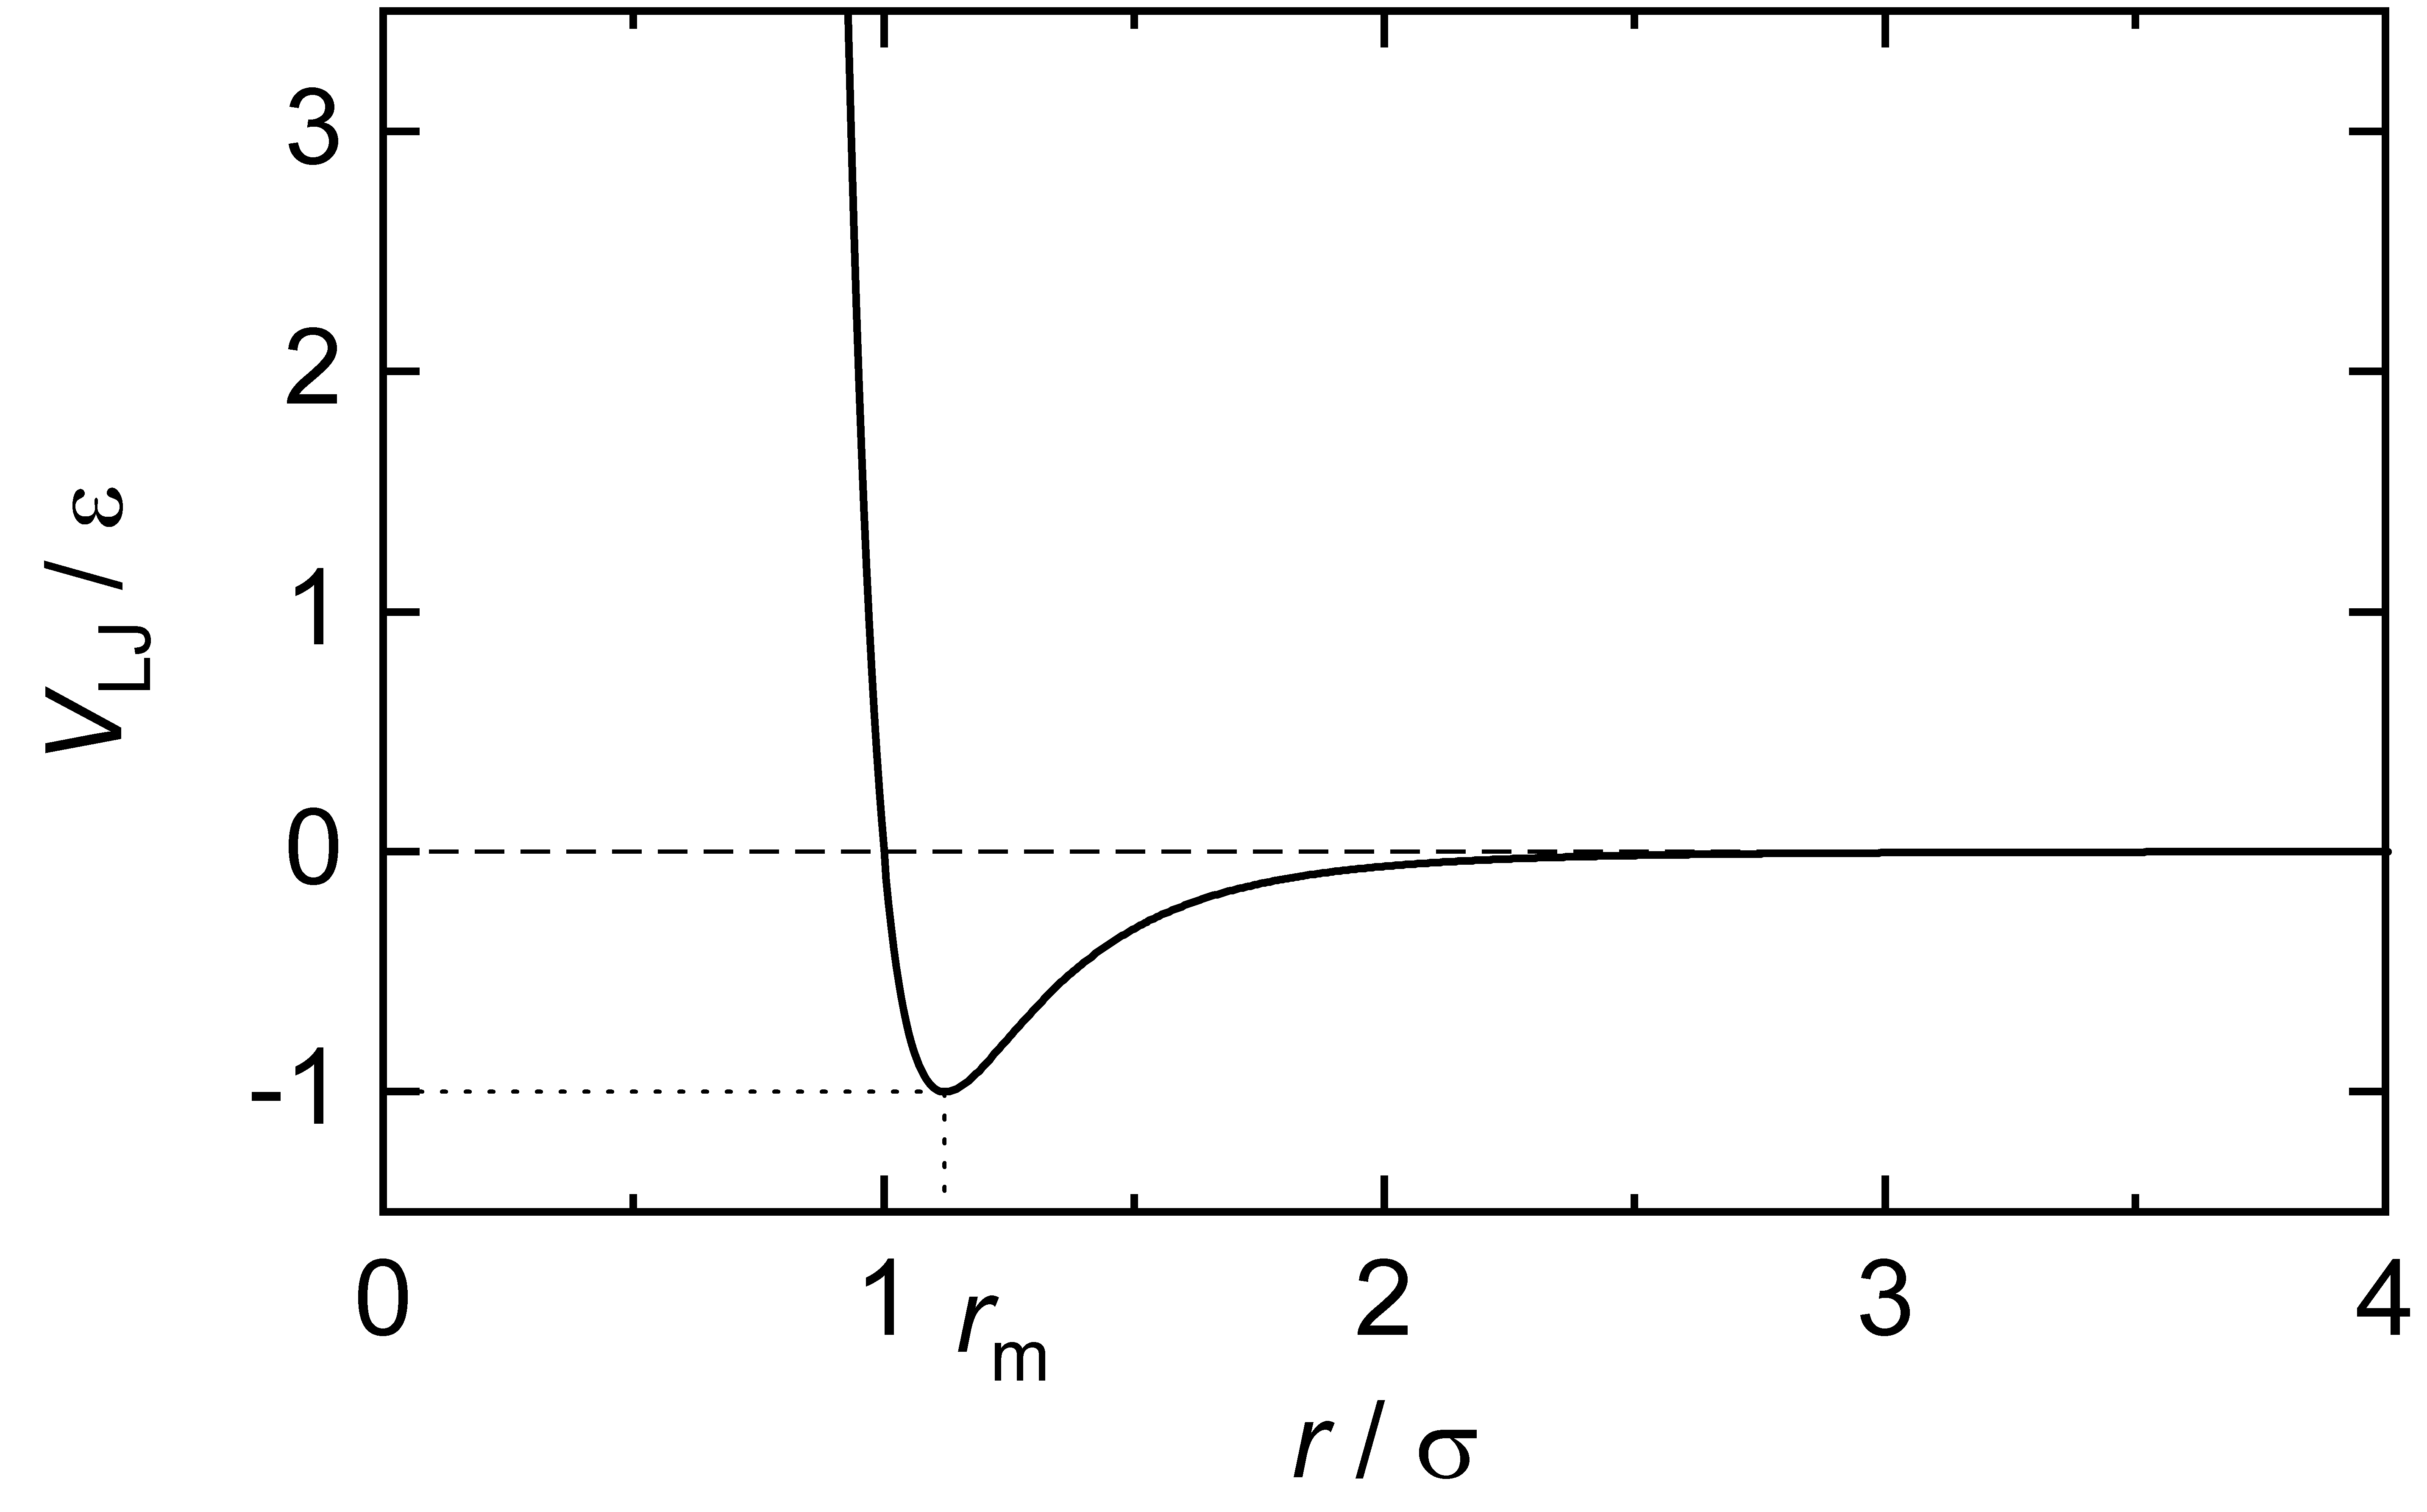
\includegraphics[height=1.00in,width=1.35in,viewport=0 0 340 270,clip]{Figures/Lennard-Jones_potential.png}
\caption{\tiny \textrm{The Lennard-Jones Potential.}}%(与文献\cite{EPJB33-47_2003}图1对比)
\label{Potential-Lennard-Jones}
\end{figure}
\vskip -20pt
	由\textrm{L-J}势改造,可以得到\textrm{WCA}势和\textrm{PHS}势}}
\item \textrm{Morse}势
	\begin{displaymath}
		U(r)=-D_{\mathrm{e}}+D_{\mathrm{e}}\bigg(1-\mathrm{e}^{-a(r-r_{\mathrm{e}})}\bigg)^2
	\end{displaymath}
	{\fontsize{7.2pt}{6.2pt}\selectfont{这里$D_{\mathrm{e}}$是\textrm{Morse}势的势阱深,参数$a$确定势阱宽度,$r_{\mathrm{e}}$是原子处于平衡位置的平衡键长
\begin{figure}[h!]
\centering
\vspace*{-0.15in}
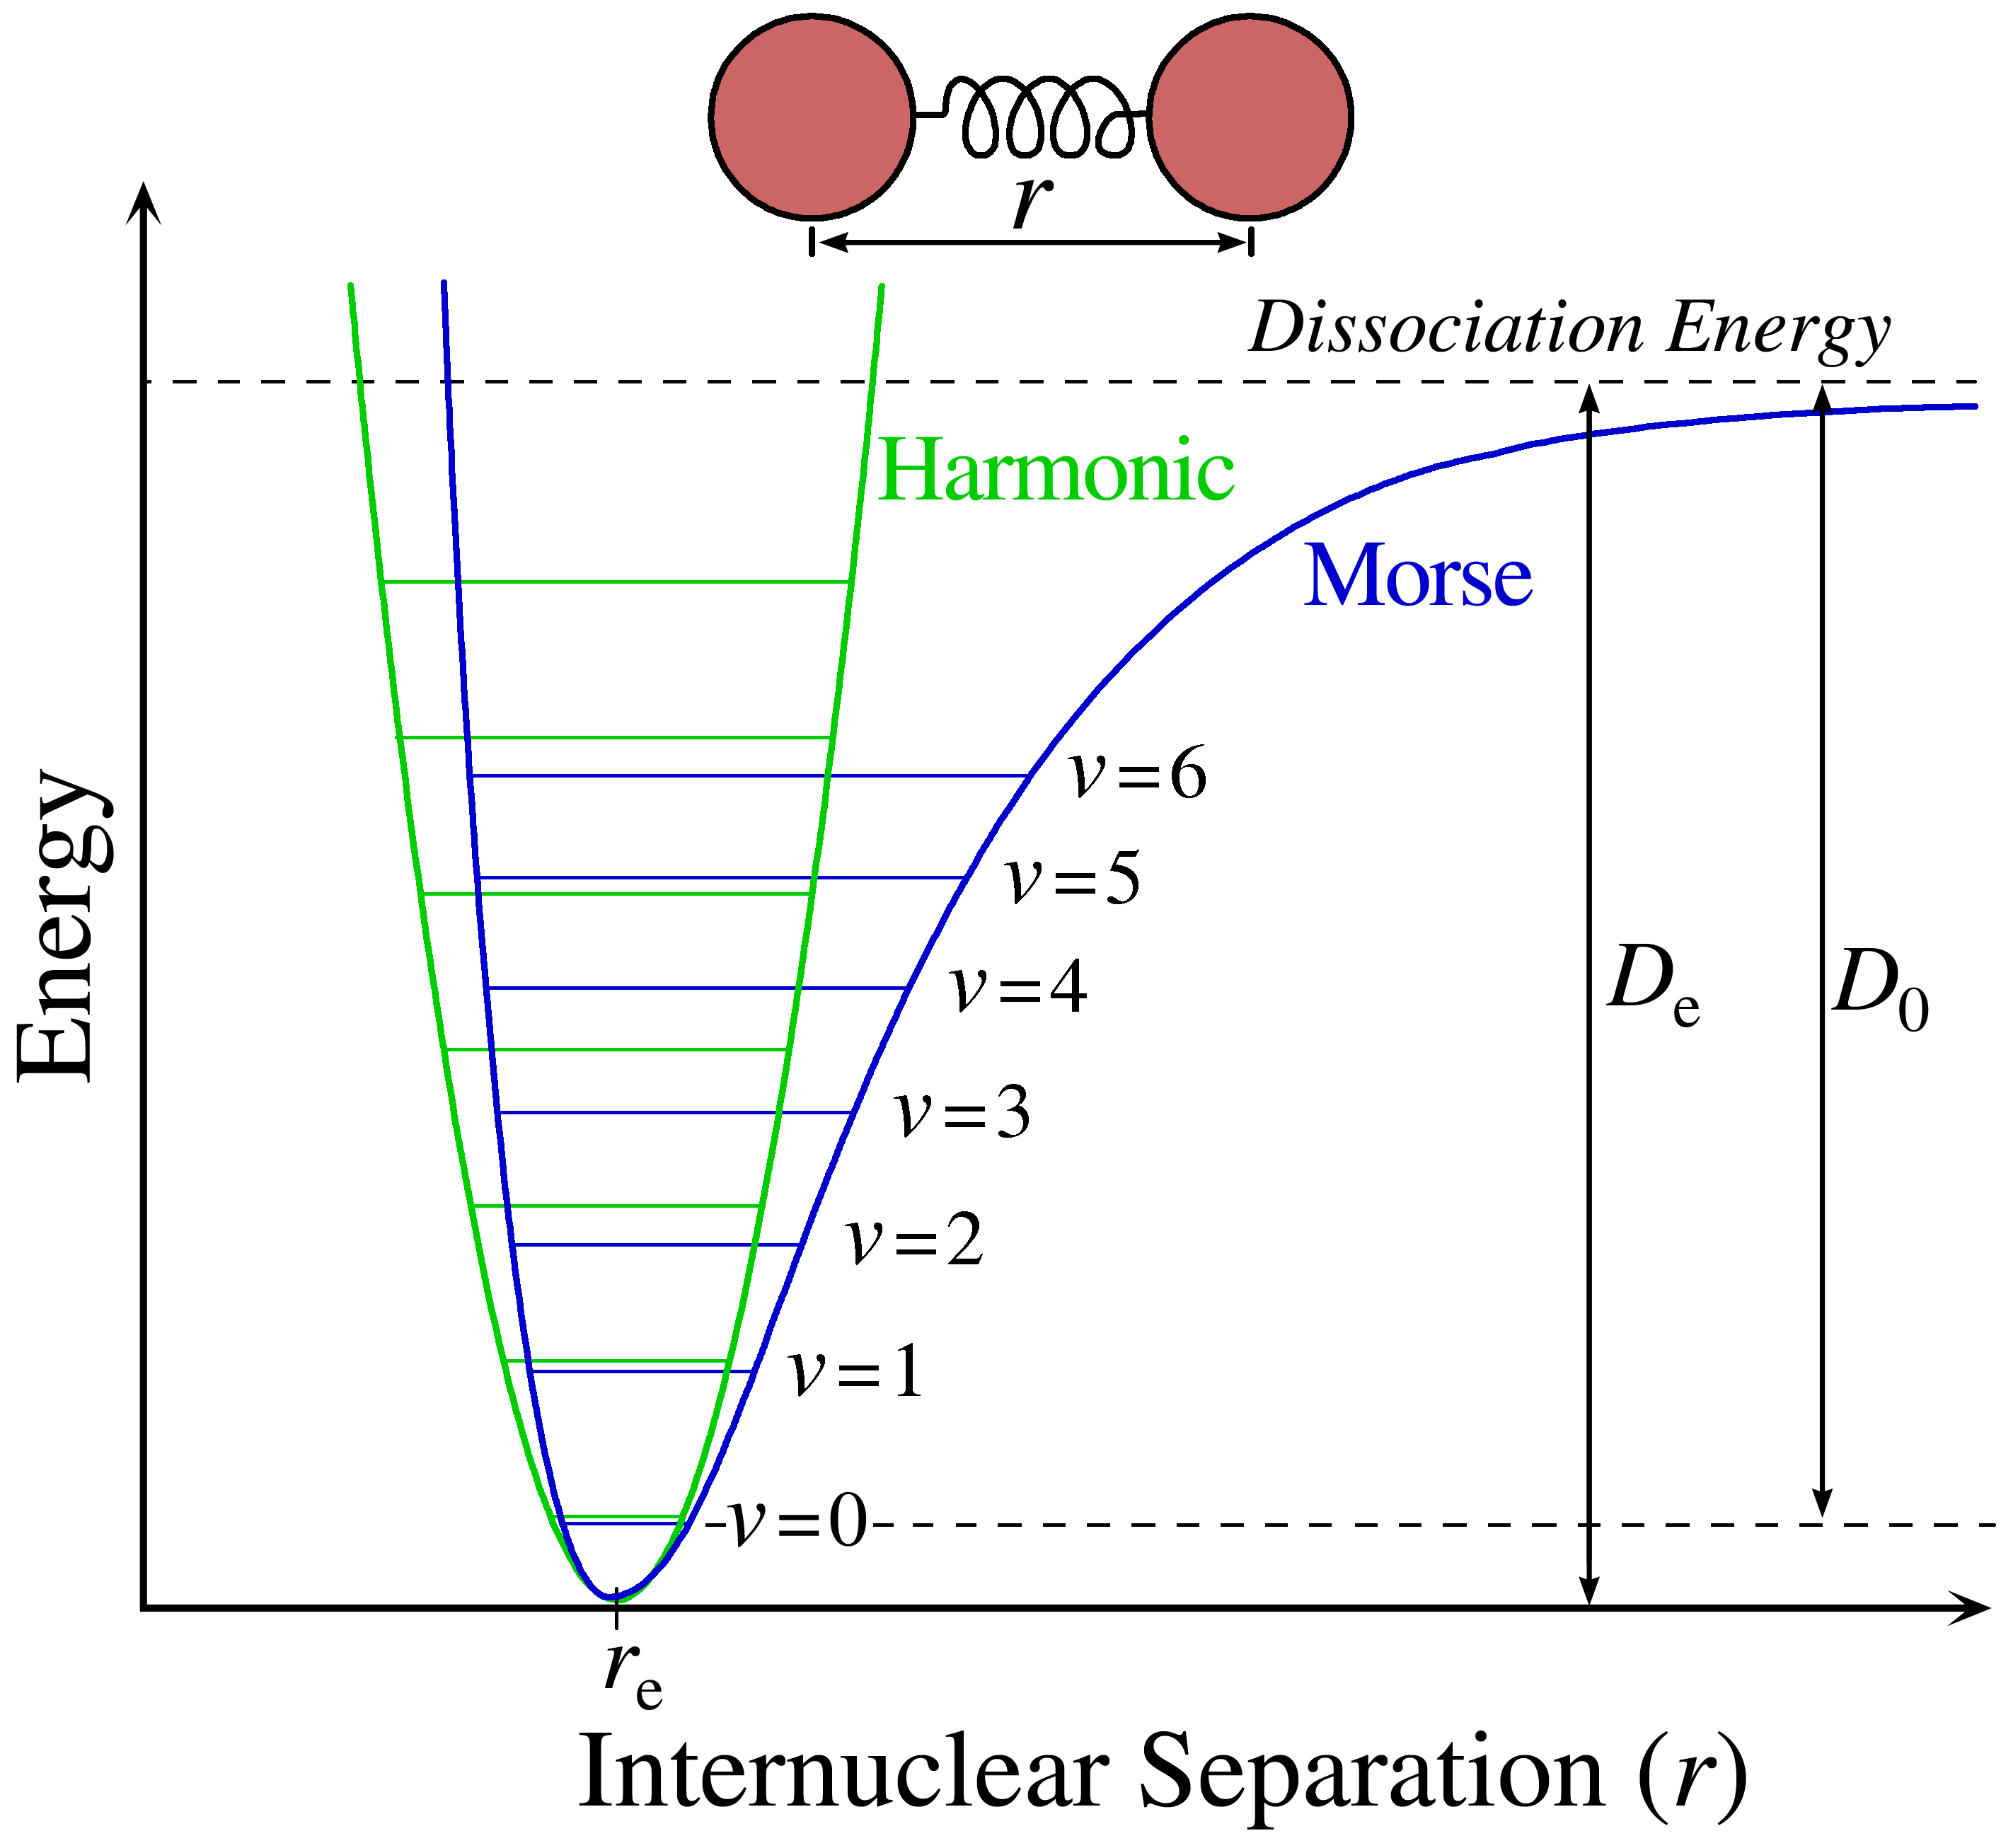
\includegraphics[height=1.30in,width=1.85in,viewport=0 0 3540 2770,clip]{Figures/Morse-potential.png}
\caption{\tiny \textrm{The Morse potential (blue) and harmonic oscillator potential (green).}}%(与文献\cite{EPJB33-47_2003}图1对比)
\label{Potential-Morse}
\end{figure}
}}
\item \textrm{EAM}势\\
	{\fontsize{7.2pt}{6.2pt}\selectfont{对于金属晶体,内能虽可以表示为对相互作用之和,但拟合原子受力非常困难:\footnote{\fontsize{5.2pt}{3.2pt}\selectfont{应用二体势计算金属弹性常数时必须涉及对体积很敏感的能量项,因为涉及缺陷、表面的体积很难确定。}}\\
	\textcolor{red}{从物理上说金属原子处于电子海洋中,电子密度来自多个原子的贡献,这是自由电子气带来的多体效应}}}\\
	\textrm{EAM}将金属中原子的势能表示为二体势和多体势之和
	\begin{displaymath}
		E_i=F_{\alpha}\bigg(\sum_{j\neq i}\rho_{\beta}(r_{ij})\bigg)+\dfrac12\sum_{j\neq i}\phi_{\alpha\beta}(\vec r_{ij})
	\end{displaymath}
	{\fontsize{7.2pt}{6.2pt}\selectfont{$\alpha$和$\beta$分别为位置$i$、$j$处的原子类型\\
		$\phi$是二体势,是原子$\alpha$和$\beta$和原子间距$r_{ij}$的函数\\
		$F$是多体势,是其余原子在位置$i$处的电荷密度与位置$i$处原子$\alpha$的相互作用能,由原子类型$\alpha$和位置$i$处的电子密度确定\\
		位置$j$原子在位置$i$处产生的电荷密度$\rho$只与位置$j$处原子类型$\beta$和原子间距$r_{ij}$有关,与方向无关
	}}\\
	各类\textrm{EAM}势中,$\phi(r)$、$\rho(r)$和$F(\rho)$都不是解析的,以数值形式存储
	\end{itemize}
}

\frame
{
	\frametitle{统计系综}
	系综(\textrm{Ensembles})是在一定的宏观条件下,由大量微观粒子组成的性质和结构完全相同的、处于各种运动状态的、各自独立的系统整体的集合\footnote{\fontsize{4.2pt}{2.2pt}\selectfont{简言之,系综是系统的集合(\textcolor{magenta}{系统}:~宏观相同,微观不同)。}}。\\
	应用\textrm{Verlet}算法,完成单粒子运动的数值积分,可以得到动力学体系的\textrm{Hamiltonian}对应的能量,进而应用统计力学的统计系综,获得宏观体系的物理量
\begin{figure}[h!]
\centering
\vspace*{-0.20in}
%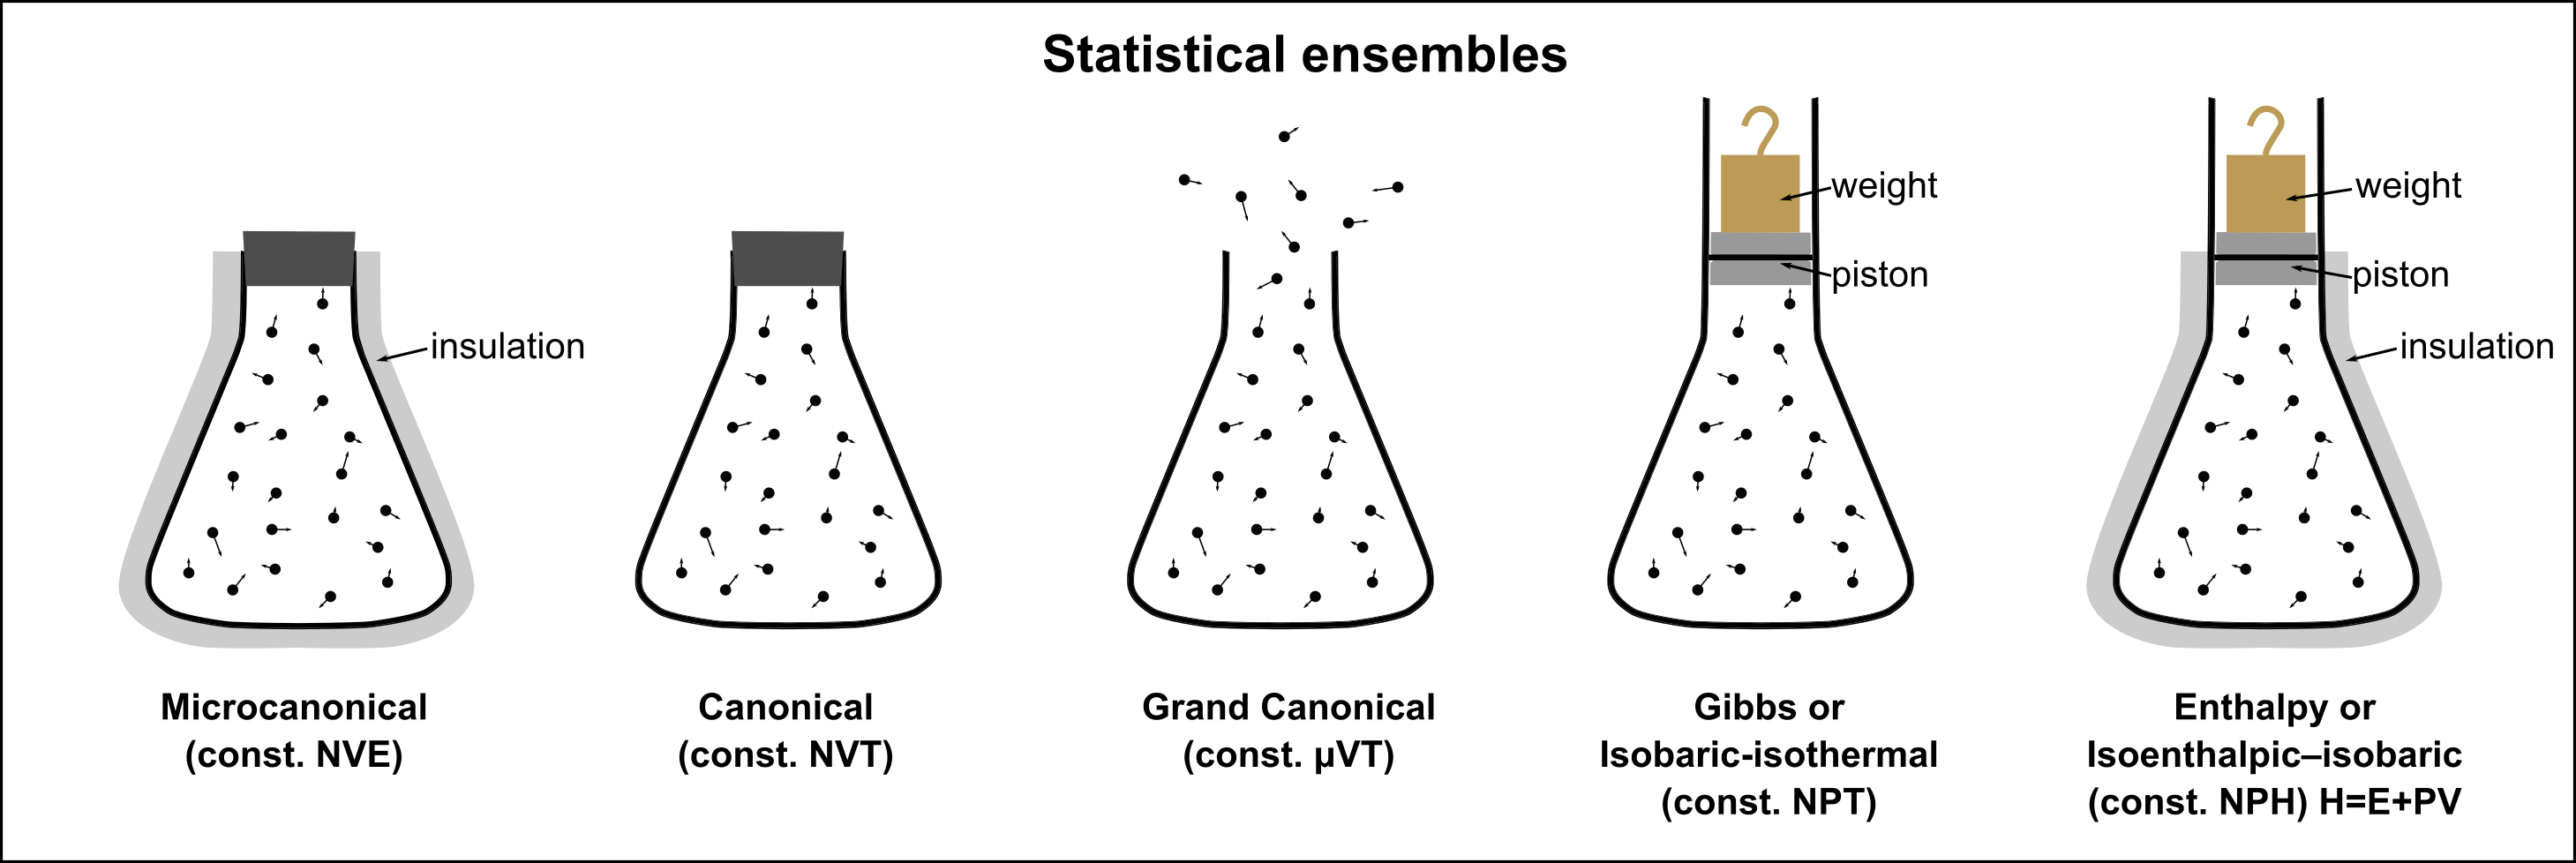
\includegraphics[height=1.60in,width=3.85in,viewport=0 0 1420 570,clip]{Figures/Statistical_Ensembles.png}
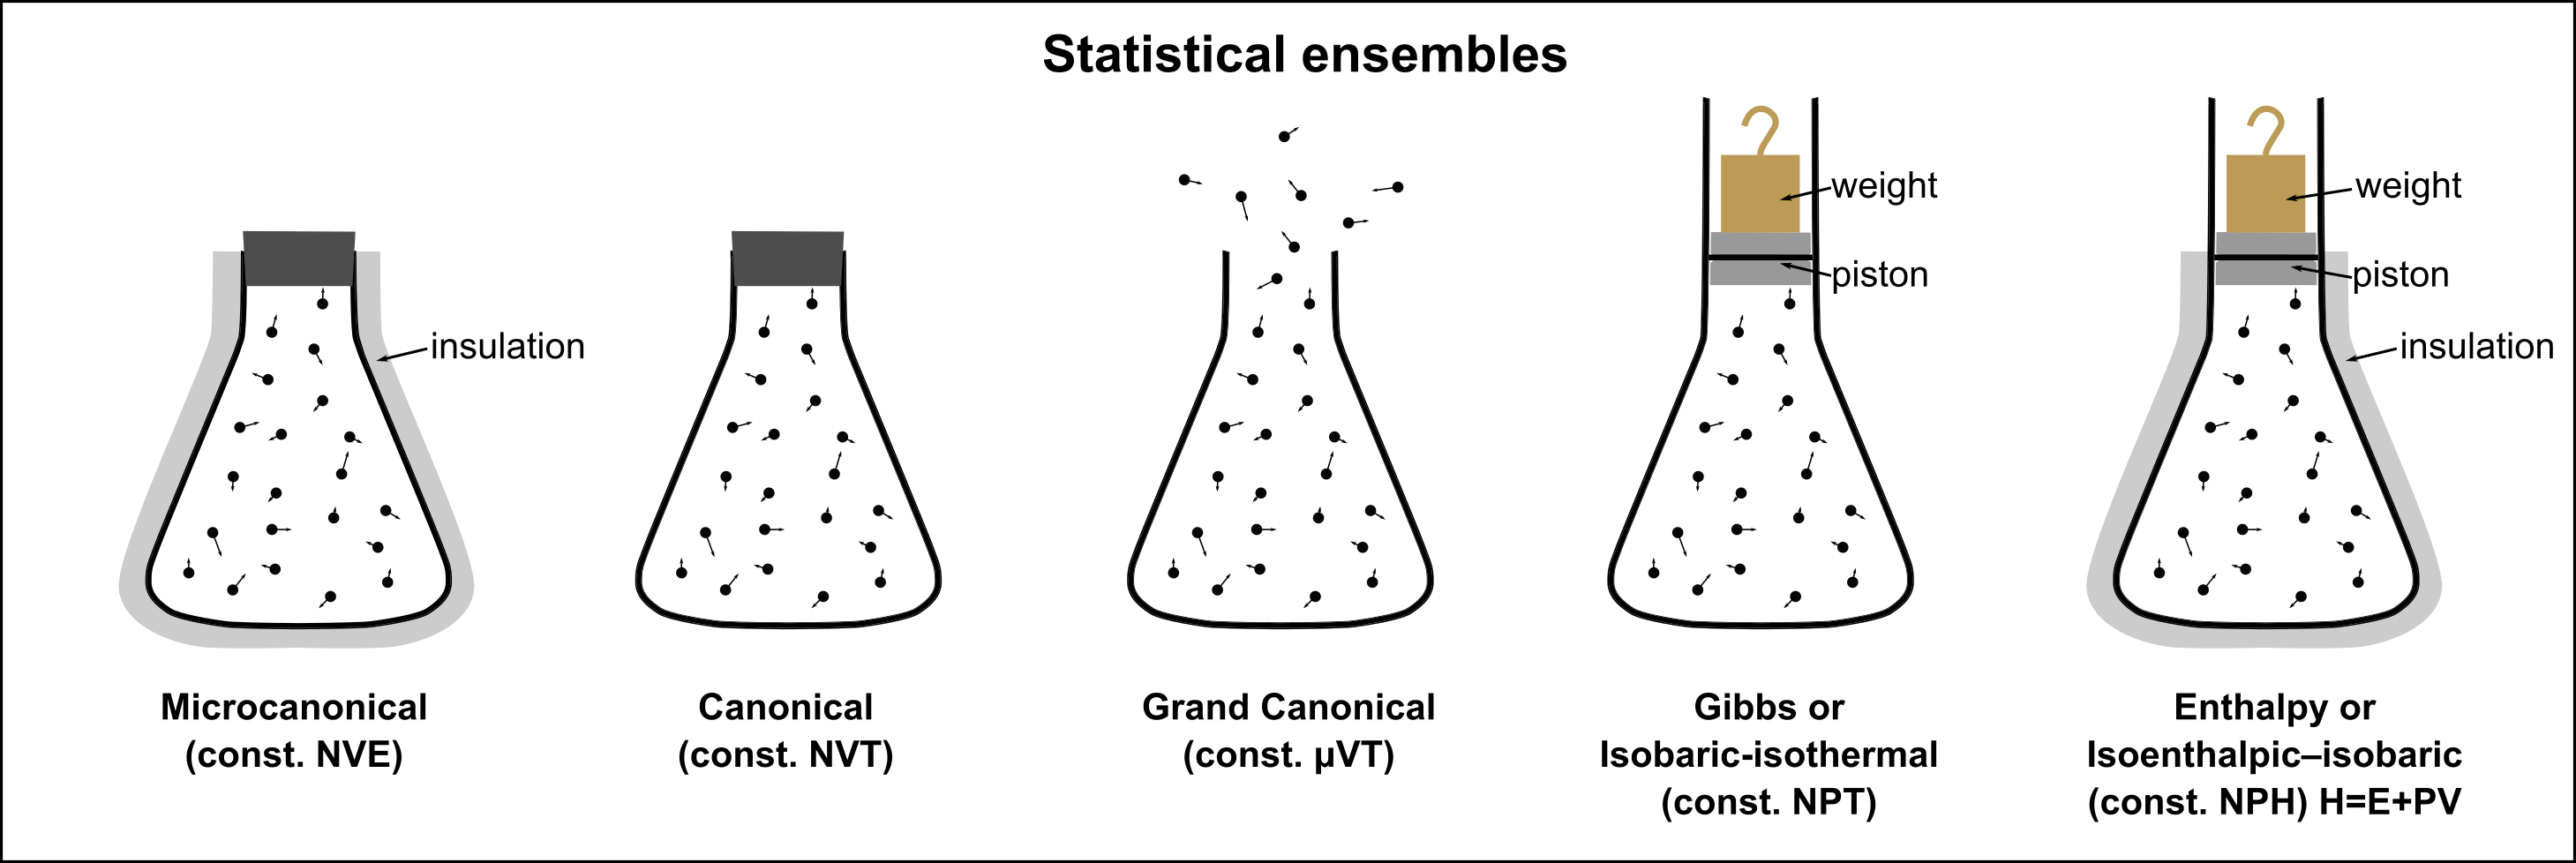
\includegraphics[height=1.30in,width=3.35in,viewport=0 0 1420 570,clip]{Figures/Statistical_Ensembles.png}
\caption{\tiny \textrm{The Statistical Ensembles.\footnote{\fontsize{3.5pt}{1.2pt}\selectfont{\textrm{canonical},汉译作“正则”,出自《楚辞\textperiodcentered 离骚》“皇揽揆余於初度兮,肇锡余以嘉名;~名余曰\textcolor{red}{正则}兮,字余曰灵均”,《楚辞章句》\upcite{Chucizhangju}:~“正,平也;~则,法也;~灵,神也;~均,调也。言正平可法则者,莫过于天;~养物均调者,莫过于地。高平曰原,故父伯庸名我为平以法天,字我为原以法地。言己上能安君,下能养民也。”,意思是说“正则”、“灵均”隐喻着某种意义,即平正是天的象征,原均是地的象征。因此正则的含义是“符合天道”,与\textrm{canonical}的意思\textrm{of, relating to, or forming a canon}意义一致。}}}}%(与文献\cite{EPJB33-47_2003}图1对比)
\label{Statistical_Ensembles}
\end{figure}
}

\subsection{第一原理分子动力学简介}
\frame
{
	\frametitle{原子间相互作用力的表示}
	分子动力学模拟中影响结果最主要因素之一是\textcolor{purple}{原子间相互作用力}的准确度
\vskip 5pt
\begin{itemize}
	\item 经典分子动力学模拟中,原子间相互作用力是根据经验势函数得到的\footnote{\fontsize{6.2pt}{4.2pt}\selectfont{经验势函数也称为力场,是参数化形式给出的原子间相互作用,一般通过对实验数据拟合或小体系的第一原理计算得到}}。构建一套高精度的经验势函数代价很高,而且经验势函数一般不具备可移植性
\end{itemize}
\vskip 5pt
	当动力学过程必须考虑量子效应(如电子影响的贡献不可忽略时),必须采用第一原理分子动力学\textrm{(Ab initio~MD,~AIMD)}
	\begin{itemize}
		\item 所谓第一原理分子动力学,就是在计算原子运动时,将电子结构变化的贡献考虑进来,因此在每一时间步长,体系实时构型下的原子受力计算,都必须伴随电子结构计算
	\end{itemize}
	一般电子结构计算采用\textrm{DFT}计算,不难想见,第一原理分子动力学模拟的代价极高
}

\frame
{
	\frametitle{第一原理分子动力学\textrm{AIMD}}
	\begin{itemize}
		\item \textrm{AIMD}将电子结构与原子和经典轨迹计算在同一基础上完成
		\item 每个原子运动步的受力都是在电子结构计算基础上获得的
%		\item 基于\textrm{B-O}近似,原子运动径迹的每一步上,电子运动都达到收敛
		\item 扩展的\textrm{Lagrangian}方法:~根据体系几何结构构造体系波函数\\
			\textcolor{blue}{\textrm{Car-Parinello}}:\\
			平面波基,构成分子轨道\\
			\textcolor{blue}{\textrm{Atom-centered Density Matrix Progation~(ADMP)}}:\\
			原子中心基,构成密度矩阵
	\end{itemize}
	\textrm{AIMD}计算内容
	\begin{itemize}
		\item 可用于复杂体系的电子结构计算
		\item 几何结构优化(能量最小化)
		\item 描述系统演化
		\item 模拟时长规模$\approx{\mathrm{ps}}(10^{-12}\mathrm{s})$~(经典分子动力学 $\approx\mathrm{ns}(10^{-9}\mathrm{s})$)
	\end{itemize}
}


\frame
{
	\frametitle{第一原理分子动力学}
	电子结构计算时,体系总能是基于\textrm{Born-Oppenheimer}近似得到,如果变化原子位置,可以得到体系总能随原子位置变化的规律\\
	作为原子位置$\vec R_i$函数的电子态总能量$E(\vec R_1,\vec R_2,\cdots,\vec R_N)$称\textcolor{red}{势能面}~(\textrm{potential surface})

	对于一套给定原子核位置$\mathbf{S}=(\vec R_1,\cdots,\vec R_N)$,$\vec R_i$表示第$i$个原子核的位置;~如果电子的基态波函数是$\psi_{\mathrm{G}}$则\\电子态能量为
	\begin{displaymath}
		E=\dfrac{\langle\psi_{\mathrm{G}}|\mathbf{H}(\mathbf{S})|\psi_{\mathrm{G}}\rangle}{\langle\psi_{\mathrm{G}}|\psi_{\mathrm{G}}\rangle}
	\end{displaymath}
作用在原子核$n$上的经典作用力,可由电子态能量对原子位置$\vec R_n$的梯度$\nabla_n$的负值给出
\begin{displaymath}
	\vec F_n=-\nabla_nE(\mathbf{S})=-\nabla_n\bigg[\dfrac{\langle\psi_{\mathrm{G}}|\mathbf{H}(\mathbf{S})|\psi_{\mathrm{G}}\rangle}{\langle\psi_{\mathrm{G}}|\psi_{\mathrm{G}}\rangle}\bigg]
\end{displaymath}
}

%\frame
%{
%	\frametitle{第一原理分子动力学的分类}
%\begin{figure}[h!]
%\centering
%\vspace*{-0.05in}
%%\hspace*{-10pt}
%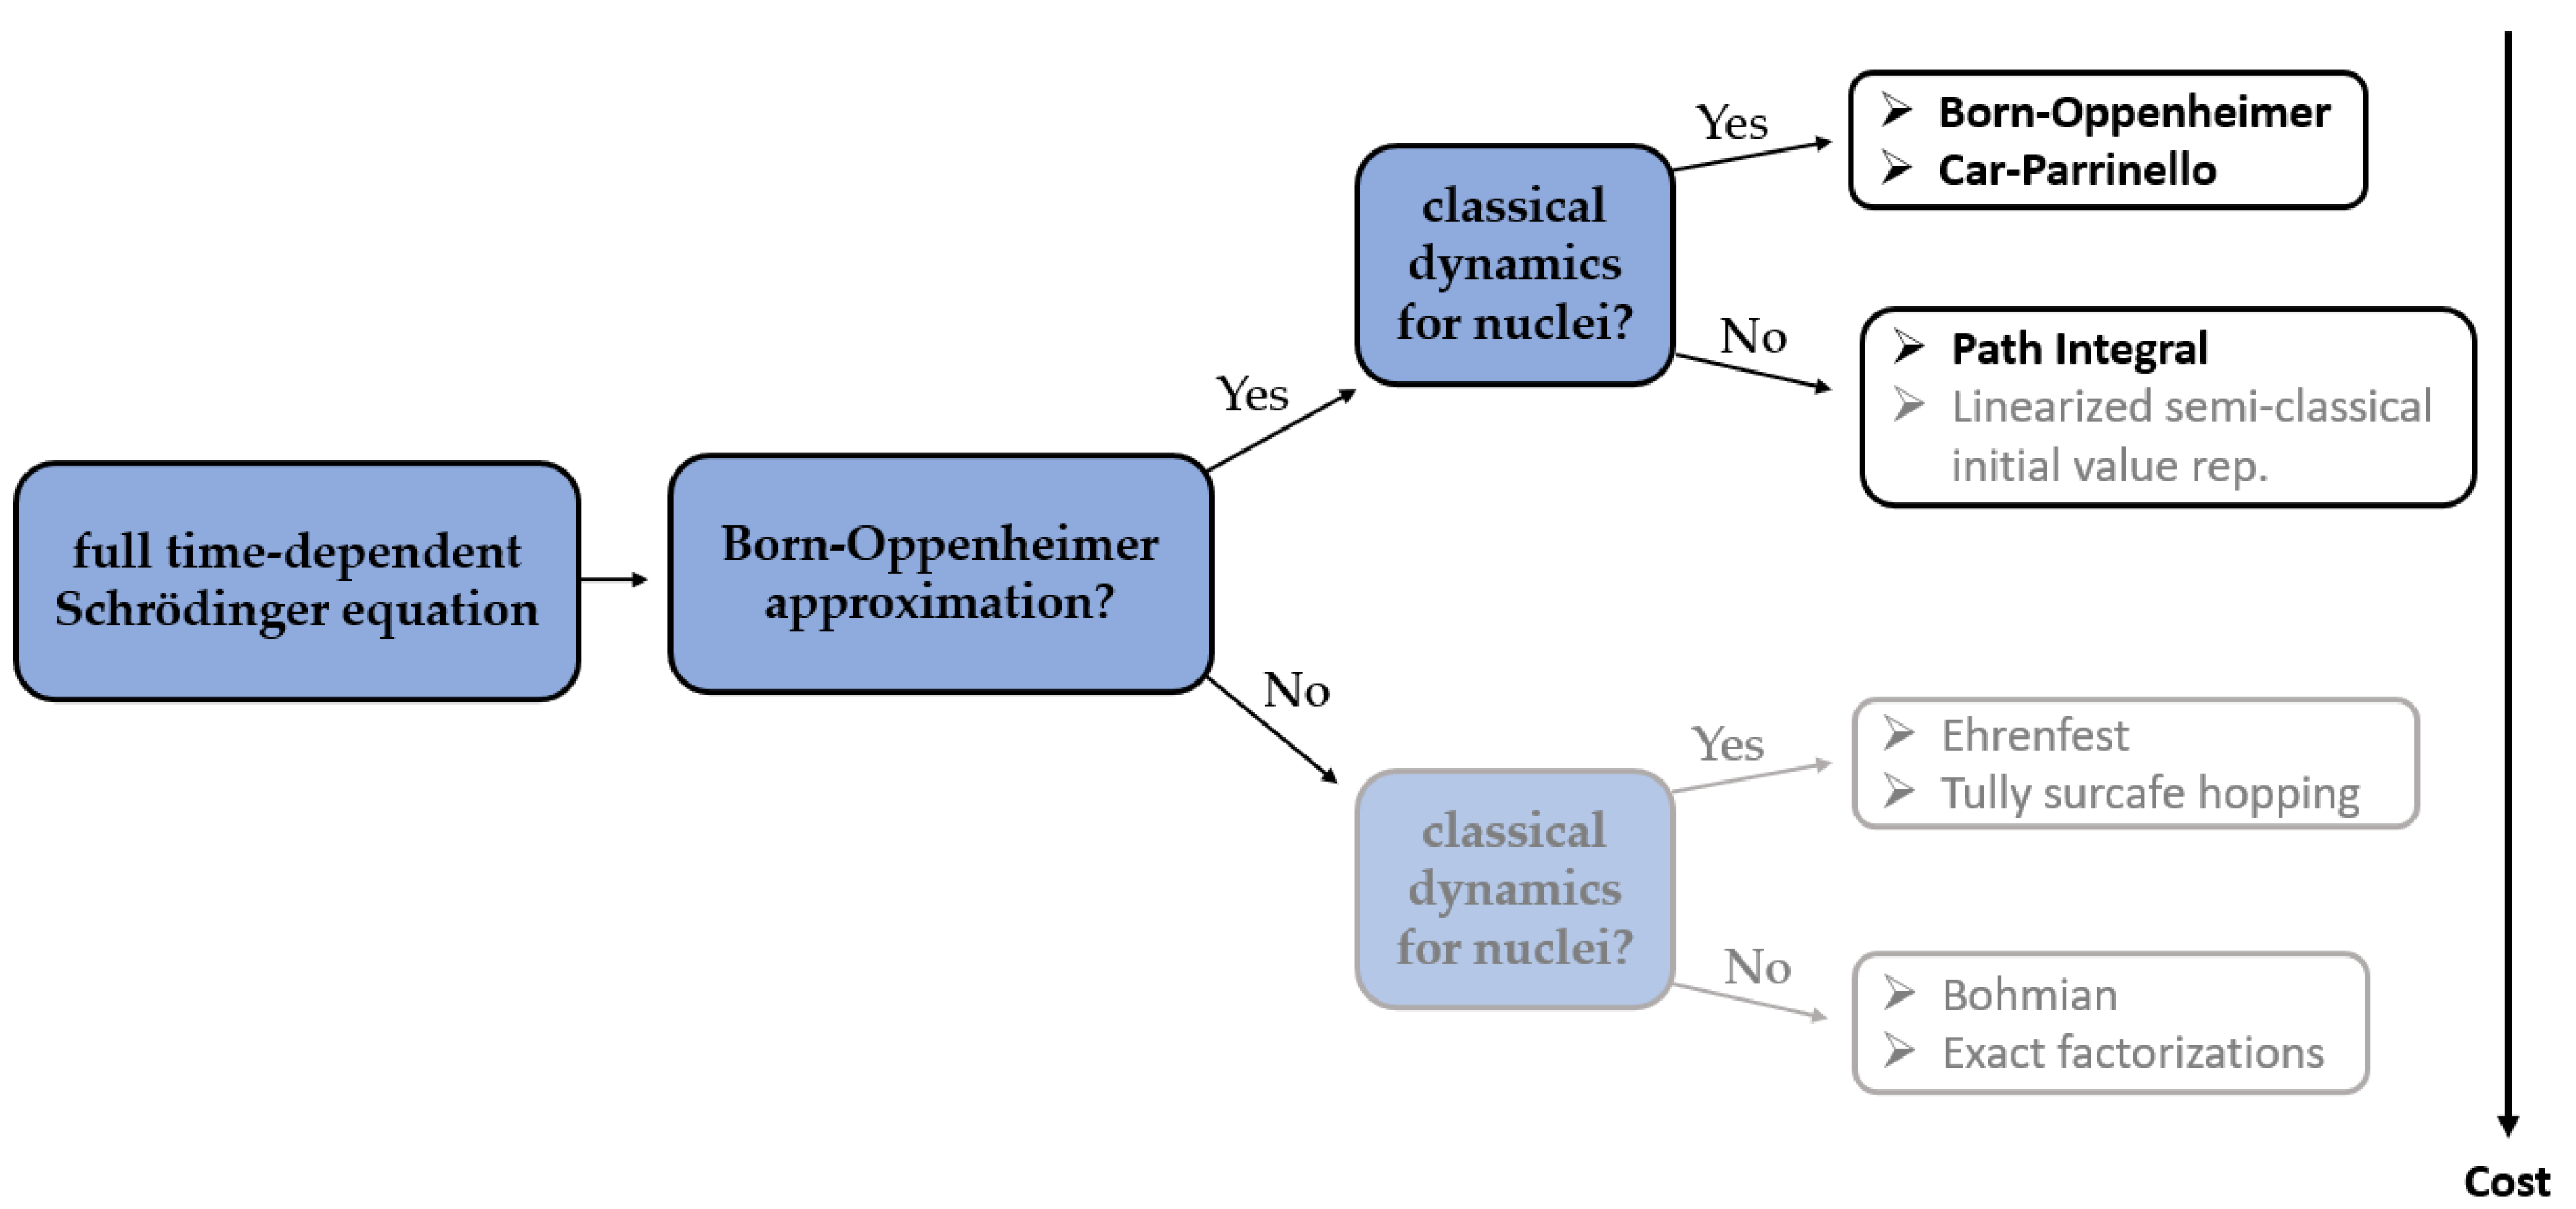
\includegraphics[height=2.3in,width=4.0in,viewport=0 0 440 230,clip]{Figures/Molecular-dynamics_Claaified.png}
%\caption{\fontsize{5.2pt}{4.2pt}\selectfont{\textrm{The major differences between the methods of aiMD simulations.}}}%
%\label{Molecular-dynamics_Claaified}
%\end{figure}
%}
%
\frame
{
	\frametitle{第一原理分子动力学中的近似}
	由于分子动力学模拟的复杂性,必须做出适当的近似。具体到第一原理分子动力学,一般有两类重要的近似:
	\begin{itemize}
		\item \textcolor{blue}{绝热近似\textrm{(adiabatic approximation)}}\\
			{\fontsize{6.2pt}{4.2pt}\selectfont{假设电子-原子核在能量层面上完全分离,彼此间没有能量传递}}
		\item \textcolor{blue}{\textrm{Born-Oppenheimer}近似}\\
			{\fontsize{6.2pt}{4.2pt}\selectfont{假设电子和原子核的运动完全解耦,对应每个时间步长的原子构型,电子可以实时处于基态\footnote{\fontsize{5.2pt}{4.2pt}\selectfont{\textrm{B-O}近似也是一种绝热近似,\textcolor{red}{但\textrm{B-O}近似下的绝热强调电子对核运动的瞬时响应}。讨论电子计算时,\textrm{B-O}近似下假设原子核是固定不动的;~在分子动力学讨论中,绝热近似强调的是电子-核运动在能量上的完整分离,而\textrm{B-O}近似则明确要求电子-核运动彼此完全解耦,且电子实时处于基态}}}}
	\end{itemize}
\begin{figure}[h!]
\centering
\vspace*{-0.25in}
%\hspace*{-10pt}
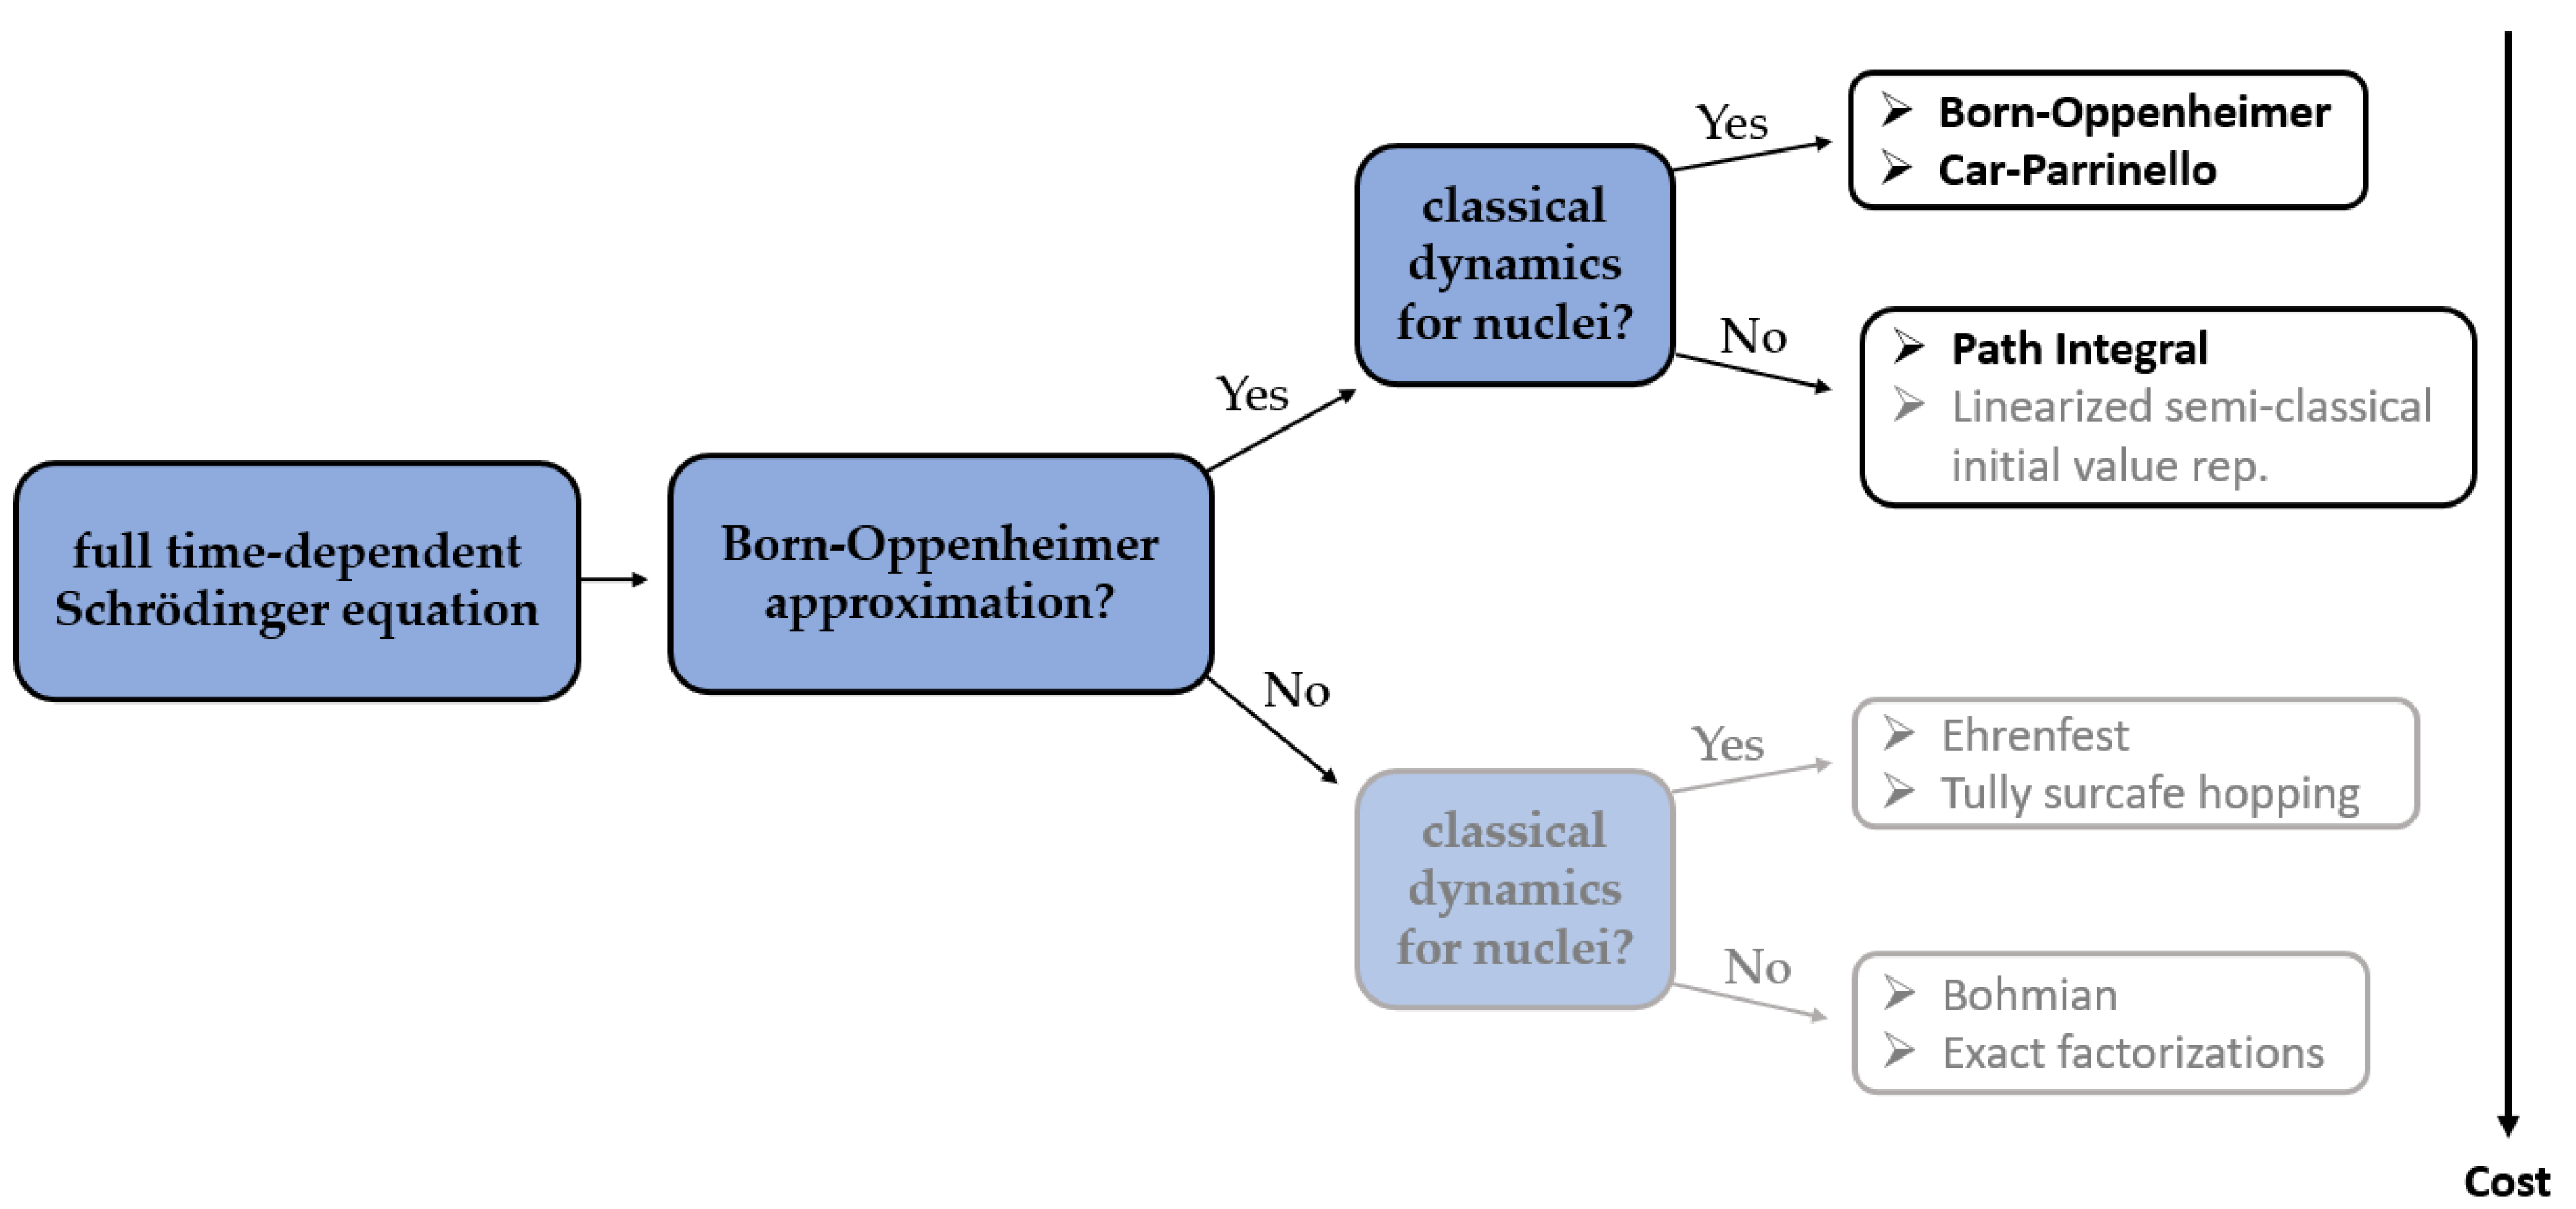
\includegraphics[height=1.55in,width=2.6in,viewport=0 0 440 230,clip]{Figures/Molecular-dynamics_Claaified.png}
%\caption{\fontsize{5.2pt}{4.2pt}\selectfont{\textrm{The major differences between the methods of aiMD simulations.}}}%
\label{Molecular-dynamics_Classified}
\end{figure}
}

\frame
{
	\frametitle{\textrm{Hellmann-Feynman}定理}
	如果$\psi_{\mathrm{G}}$是\textrm{Hamiltonian}的本征态,有
	\begin{displaymath}
		\begin{aligned}
			&(\langle\psi_{\mathrm{G}}|\psi_{\mathrm{G}}\rangle)^2\nabla_nE\\
			=&\big[\langle(\nabla_n\psi_{\mathrm{G}}|\mathbf{H}|\psi_{\mathrm{G}}\rangle+\langle\psi_{\mathrm{G}}|(\nabla_n\mathbf{H})|\psi_{\mathrm{G}}\rangle+\langle\psi_{\mathrm{G}}|\mathbf{H}|(\nabla_n\psi_{\mathrm{G}})\rangle\big]\langle\psi_{\mathrm{G}}|\psi_{\mathrm{G}}\rangle\\
			&-\langle\psi_{\mathrm{G}}|\mathbf{H}|\psi_{\mathrm{G}}\rangle\big[\langle(\nabla_n\psi_{\mathrm{G}})|\psi_{\mathrm{G}}\rangle+\langle\psi_{\mathrm{G}}|(\nabla_n\psi_{\mathrm{G}})\rangle\big]
		\end{aligned}
	\end{displaymath}
	{\fontsize{6.2pt}{5.2pt}\selectfont{这里暂不考虑$\mathbf{H}$对原子核位置$\mathbf{S}$的依赖}}\\
	\vskip 5pt
	\textrm{Hellmann-Feynman}定理指出:~如果\textrm{Hamiltonian}量$\mathbf{H}$是\textrm{Hermitian}的,并且有
	\begin{displaymath}
		\mathbf{H}\psi_{\mathrm{G}}=E_{\mathrm{G}}\psi_{\mathrm{G}}
	\end{displaymath}
则上述表达式中,除了$\langle\psi_{\mathrm{G}}|(\nabla_n\mathbf{H})|\psi_{\mathrm{G}}\rangle$之外,等式右侧其余各项彼此抵消。由此得到能量梯度的表达式
\begin{displaymath}
	\nabla_nE=\dfrac{\langle\psi_{\mathrm{G}}|(\nabla_n\mathbf{H})|\psi_{\mathrm{G}}\rangle}{\langle\psi_{\mathrm{G}}|\psi_{\mathrm{G}}\rangle}
\end{displaymath}
}

\frame
{
	\frametitle{第一原理分子动力学:~\textrm{BOMD}}
	如果绝热近似和\textrm{Born-Oppenheimer}近似同时满足,称为\textrm{Born-Oppenheimer}分子动力学\textrm{(BOMD)}
	\begin{itemize}
		\item 原子核运动的势函数为$E[\{\psi_i\};\mathbf{R}]$,并且每个时间步长内,势函数对$\{\psi_i(\vec r)\}$取极小值\\
			\begin{displaymath}
				\begin{aligned}
					L_{\mathrm{BO}}(\{\psi_i\};~\mathbf{R},\dot{\mathbf{R}})=&\dfrac12\sum_{I=1}^NM_I\dot{\mathbf{R}}^2_I-\underset{\{\psi_i\}}{\textcolor{red}{\min}}~E[\{\psi_i\};\mathbf{R}]\\
					&+\sum_{ij}\Lambda_{ij}(\langle\psi_i|\psi_j\rangle-\delta_{ij})
				\end{aligned}
			\end{displaymath}
		\item 运动方程\textrm{(Equations of Motion,~EOM)}
			\begin{displaymath}
				\begin{aligned}
					\hspace*{-40pt}
					M_I\ddot{\mathbf{R}}_I=&-\nabla_{\mathbf{R}_I}\bigg[\underset{\{\psi_i\}}{\textcolor{red}{\min}}~E[\{\psi_i\};\mathbf{R}]\bigg|_{\{\langle\psi_i|\psi_j\rangle=\delta_{ij}\}}\bigg]\\
					=&\textcolor{purple}{-\dfrac{\partial E}{\partial\mathbf{R}_I}}\textcolor{blue}{+\sum_{i,j}\Lambda_{ij}\dfrac{\partial}{\partial \mathbf{R}_I}\langle\psi_i|\psi_j\rangle}\textcolor{magenta}{-2\sum_i\dfrac{\partial\langle\psi_i|}{\partial\mathbf{R}_I}\bigg[\dfrac{\delta E}{\delta\langle\psi_i|}-\sum_j\Lambda_{ij}|\psi_j\rangle\bigg]}
				\end{aligned}
			\end{displaymath}
	\end{itemize}
}

\frame
{
	\frametitle{第一原理分子动力学:~\textrm{BOMD}}
	\begin{itemize}
		\item $\textcolor{purple}{\dfrac{\partial E}{\partial\mathbf{R}_I}}$表示\textrm{Hellmann-Feynman}力$\vec F_{\mathrm{HF}}$
		\item $\textcolor{blue}{\sum\limits_{i,j}\Lambda_{ij}\dfrac{\partial}{\partial \mathbf{R}_I}\langle\psi_i|\psi_j\rangle}$是\textrm{Pulay}力$\vec F_{\mathrm{WF}}$\\
			{\fontsize{6.2pt}{4.2pt}\selectfont{源于电子波函数正交要求,且只有当基函数为局域函数(依赖于$\mathbf{R}$时)才有贡献}}
		\item $\textcolor{magenta}{\sum\limits_i\dfrac{\partial\langle\psi_i|}{\partial\mathbf{R}_I}\bigg[\dfrac{\delta E}{\delta\langle\psi_i|}-\sum\limits_j\Lambda_{ij}|\psi_j\rangle\bigg]}$表示非自洽电子态的影响$\vec F_{\mathrm{NSC}}$\\
			{\fontsize{6.2pt}{4.2pt}\selectfont{源自非局域基(如平面波),由于波函数非显式依赖$\mathbf{R}$,因此展开系数$c_{ij}(\mathbf{R})$依赖于原子核位置
			\begin{displaymath}
				\psi_i(\mathbf{R})=\sum\limits_jc_{ij}(\mathbf{R})\phi_i
			\end{displaymath}
			前面\textrm{MOE}中的系数\textrm{2}源于\textrm{K-S}轨道波函数为实数时的简化表示\\
			这一项的贡献比起$F_{\mathrm{HF}}$小很多,\textcolor{blue}{只要当$\psi_i(\mathbf{R})$是体系精确的电子的本征态波函数,该项就会消失}——换言之,只有非完全自洽的电子计算,才需要考虑该项的贡献。显然,所有数值计算中,都将存在不等式
	\begin{displaymath}
			0\leqslant-\dfrac{\delta E}{\delta\langle\psi_i|}+\sum_j\Lambda_{ij}|\psi_j\rangle=-\hat{H_{\mathrm{e}}}\langle\psi_j|+\sum_j\Lambda_{ij}|\psi_j\rangle
		\end{displaymath} }}
	\end{itemize}
}

\frame
{
	\frametitle{第一原理分子动力学:~\textrm{BOMD}}
	另一方面,如果忽略$\vec F_{\mathrm{WF}}$和$\vec F_{\mathrm{NSC}}$的贡献,仅对体系电子的非本征态波函数应用\textrm{Hellmann-Feynman}定理,得到的结果和精确计算的原子受力
	\begin{displaymath}
		\vec F=\vec F_{\mathrm{HF}}+\vec F_{\mathrm{WF}}+\vec F_{\mathrm{NSC}}
	\end{displaymath}
	计算相比,也只有微小的偏差
	\vskip 1.5pt
	这是因为在\textrm{DFT}框架下,能量是电荷密度的非线性函数,因此$H_{\mathrm{e}}$必须通过迭代求解;~而原子受力的误差则随电荷密度线性变化——这也解释了为什么一般\textrm{BOMD}计算的原子受力比体系总能要精确得多

	\vskip 5pt
	在\textrm{BOMD}中,\textrm{Born-Oppenheimer}近似下核与电子的运动完全解耦,在此基础上考虑绝热近似,将不再有对动力学模拟的时间步长限制,相比于其它\textrm{AIMD}方法,\textrm{BOMD}模拟允许的时间步长要长得多
}

\frame
{
	\frametitle{第一原理分子动力学:~\textrm{CPMD}}
	1985年\textrm{Car}和\textrm{Parrinello}在密度泛函理论基础上,将第一原理方法应用到分子动力学研究中,形成\textrm{Car-Parrinello Molecular dynamics~(CPMD)}
	\begin{itemize}
		\item 与\textrm{BOMD}不同,在\textrm{CPMD}中,电子自由度存在于经典\textrm{Lagrangian}中
			\begin{displaymath}
				\begin{aligned}
					L_{\mathrm{CP}}(\{\psi_i\};~\mathbf{R},\dot{\mathbf{R}})=&\textcolor{blue}{\dfrac12\mu\sum_i\langle\dot{\psi}_i|\dot{\psi}_i\rangle}+\dfrac12\sum_{I=1}^NM_I\dot{\mathbf{R}}^2_I\\
					-&\textcolor{red}{E}[\{\psi_i\};\mathbf{R}]\\
					&+\sum_{ij}\Lambda_{ij}(\langle\psi_i|\psi_j\rangle-\delta_{ij})
				\end{aligned}
			\end{displaymath}
			{\fontsize{6.2pt}{4.2pt}\selectfont{在经典\textrm{Lagrangian}中考虑电子自由度,人为地引入了傀电子质量参数$\mu$和傀轨道速度$\dot{\psi}_i$}}
	\end{itemize}
}

\frame
{
	\frametitle{第一原理分子动力学:~\textrm{CPMD}}
	\begin{itemize}
		\item \textrm{CPMD}下的运动方程表示为
			\begin{displaymath}
				\begin{aligned}
					M_I\ddot{\mathbf{R}}_I=&-\nabla_{\mathbf{R}_I}\bigg[E[\{\psi_i\};\mathbf{R}]\bigg|_{\{\langle\psi_i|\psi_j\rangle=\delta_{ij}\}}\bigg]\\
					=&\textcolor{purple}{-\dfrac{\partial E}{\partial\mathbf{R}_I}}\textcolor{blue}{+\sum_{i,j}\Lambda_{ij}\dfrac{\partial}{\partial \mathbf{R}_I}\langle\psi_i|\psi_j\rangle}\\
					\mu\ddot{\psi}_i(\vec r,t)=&-\dfrac{\delta E}{\delta\langle\psi_i|}+\sum_j\Lambda_{ij}|\psi_j\rangle\\
					=&-\hat{H_{\mathrm{e}}}\langle\psi_j|+\sum_j\Lambda_{ij}|\psi_j\rangle
				\end{aligned}
			\end{displaymath}
			{\fontsize{6.2pt}{4.2pt}\selectfont{$-\dfrac{\delta E}{\delta\langle\psi|}$表示经典力学框架下的电子受力,用来描述分子动力学范畴内电子自由度随原子核运动的情况 }}
	\end{itemize}
}

\frame
{
	\frametitle{\textrm{CPMD}计算的特点}
	\begin{itemize}
		\item 计算成本大大节约\\
			{\fontsize{8.2pt}{4.2pt}\selectfont{相比于\textrm{BOMD},\textrm{CPMD}无需在每个分子动力学时间步长执行电子自洽计算}}
		\item 计算时间步长不能太长\\
			{\fontsize{8.2pt}{4.2pt}\selectfont{绝热近似要求电子-核运动能量彼此分离,\textcolor{blue}{声子最高频率}$\omega_{\mathrm I}$必须远小于\textcolor{blue}{傀电子最低振动频率}$\omega_{\mathrm e}$
			\begin{displaymath}
				\omega_{\mathrm e}\propto\sqrt{\dfrac{\Delta E_{\mathrm{gap}}}{\mu}}
			\end{displaymath}
			$\Delta E_{\mathrm{gap}}$是\textrm{K-S}单粒子的带隙,许可最大时间步长$\Delta t_{\mathrm{max}}<1/\omega_{\mathrm{e}}$,大小主要由$\sqrt{\mu}$}}确定
		\item $\mu$物理上没有意义,但通过调节$\mu$可以平衡\textrm{AIMD}的效率和精度,一般选取$\mu$使得$\omega_{\mathrm{I}}<<\omega_{\mathrm{I}}$成立
		\item 对于金属/导体的\textrm{CPMD}计算,由于$\Delta E_{\mathrm{gap}}=0$,必须要求体系通过恒温条件平衡交换能或者泛函允许分数占据
		\end{itemize}
}

\frame
{
	\frametitle{其它\textrm{AIMD}:~\textrm{PIMD}和\textrm{Ehrenfest~MD}}
	\begin{itemize}
		\item \textrm{Path Integral~MD~(PIMD)}\footnote{\fontsize{6.2pt}{4.2pt}\selectfont{基于量子统计的第一原理路径积分称为\textrm{Feynman}路径积分\textrm{(path integrals)}}}\\
			\textrm{PIMD}用量子力学计算电子和原子核运动,因此该方法比\textrm{BOMD}和\textrm{CPMD}方法精确,特别是对于含有轻元素体系——计算量也要大得多
		\item \textrm{Ehrenfest~MD}\\
			电子自由度通过求解含时\textrm{(Time-dependent)~Schr\"odinger}方程得到,当$\Delta t\rightarrow0$,自由度变化对应于电子的幺正传播\textrm{(unitary propagation)}\footnote{\fontsize{6.2pt}{4.2pt}\selectfont{\textrm{Ehrenfest~MD}的幺正变换确保波函数保持正交,但代价是积分时间步长必须极小,因此\textrm{Ehrenfest~MD}模拟时间尺度仅达\textrm{atto}$(10^{-18})$秒尺度}}
	\end{itemize}
	\textcolor{blue}{\textrm{CPMD}结合了\textrm{BOMD}与\textrm{Ehrenfest~MD}的优点}:
	\begin{itemize}
		\item 计算体系受力由总能对粒子位置的求导,并非求电子态的$\langle\Psi_0|\hat H_{\mathrm{e}}|\Psi_0\rangle$极小值
		\item 因为选择平面波基,$\vec F_{\mathrm{NSC}}$自然为0
	\end{itemize}
}

\frame
{
	\frametitle{平衡态统计基础}
	系综(\textrm{Ensembles})是在一定的宏观条件下,由大量微观粒子组成的性质和结构完全相同的、处于各种运动状态的、各自独立的系统整体的集合。简言之,系综是给定宏观条件下,所有微观状态的集合。
%	应用\textrm{Verlet}算法,完成单粒子运动的数值积分,可以得到动力学体系的\textrm{Hamiltonian}对应的能量,进而应用统计力学的统计系综,获得宏观体系的物理量
	\vskip 3pt
	\textcolor{blue}{等概率原理}\textrm{(Principle of equal weights)}:\\
	一个热力学体系有相同的概率到达每个可能经历的微观态。\\
	等概率原理导出\textrm{Boltzmann}分布
	\begin{displaymath}
		P_j=\dfrac{\mathrm{e}^{-\beta\varepsilon_j}}Q
	\end{displaymath}
	这里$Q$称为配分函数\textrm{(partition function)}
	\begin{displaymath}
		\begin{aligned}
			Q=&\sum_i\mathrm{e}^{(-\beta\varepsilon_i)}\\
			\beta=&1/k_{\mathrm{B}}T
		\end{aligned}
	\end{displaymath}
	物理量的系综平均
	\begin{displaymath}
		\langle A\rangle=\sum_jA_j\mathrm{e}^{(-\beta\varepsilon_j)}/Q
	\end{displaymath}
}

\frame
{
	\frametitle{常用统计系综}
\begin{figure}[h!]
\centering
\vspace*{-0.20in}
%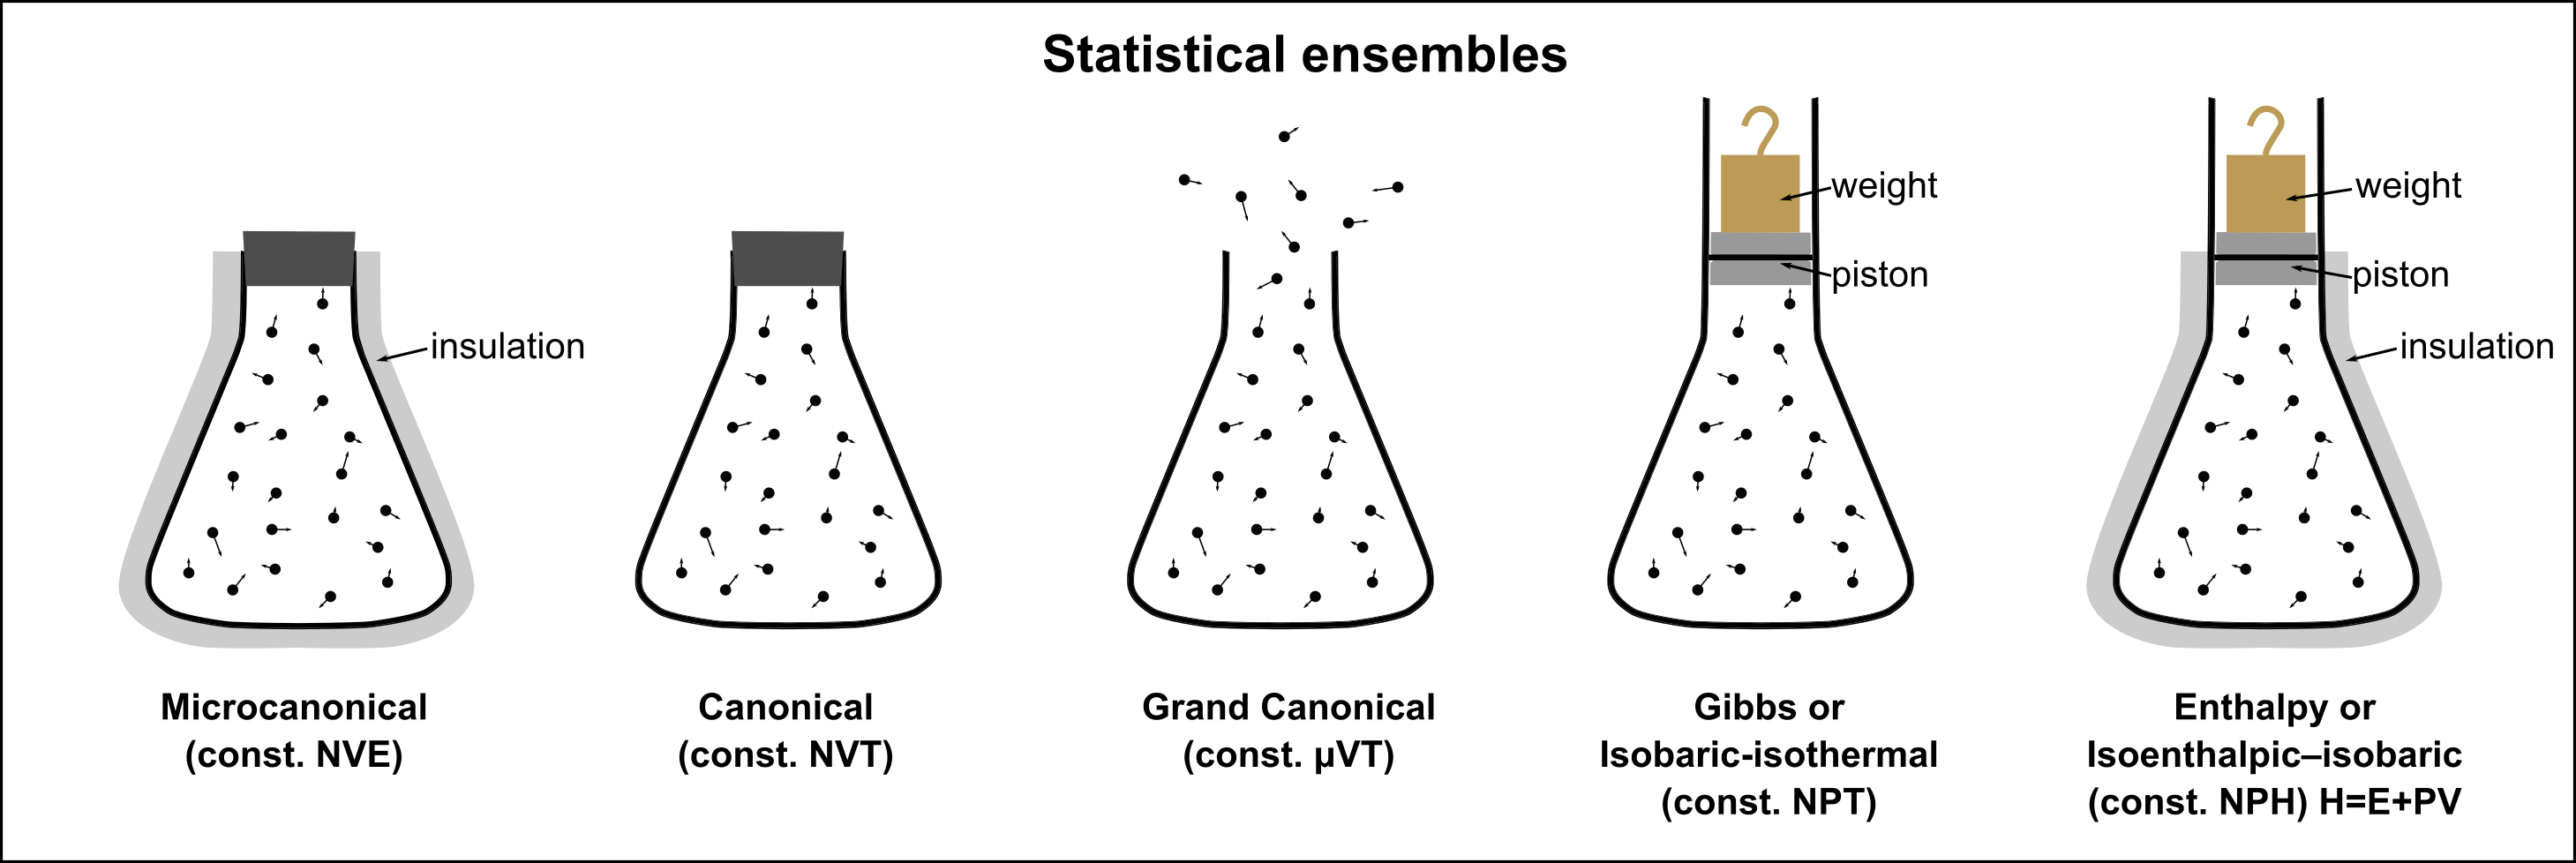
\includegraphics[height=1.60in,width=3.85in,viewport=0 0 1420 570,clip]{Figures/Statistical_Ensembles.png}
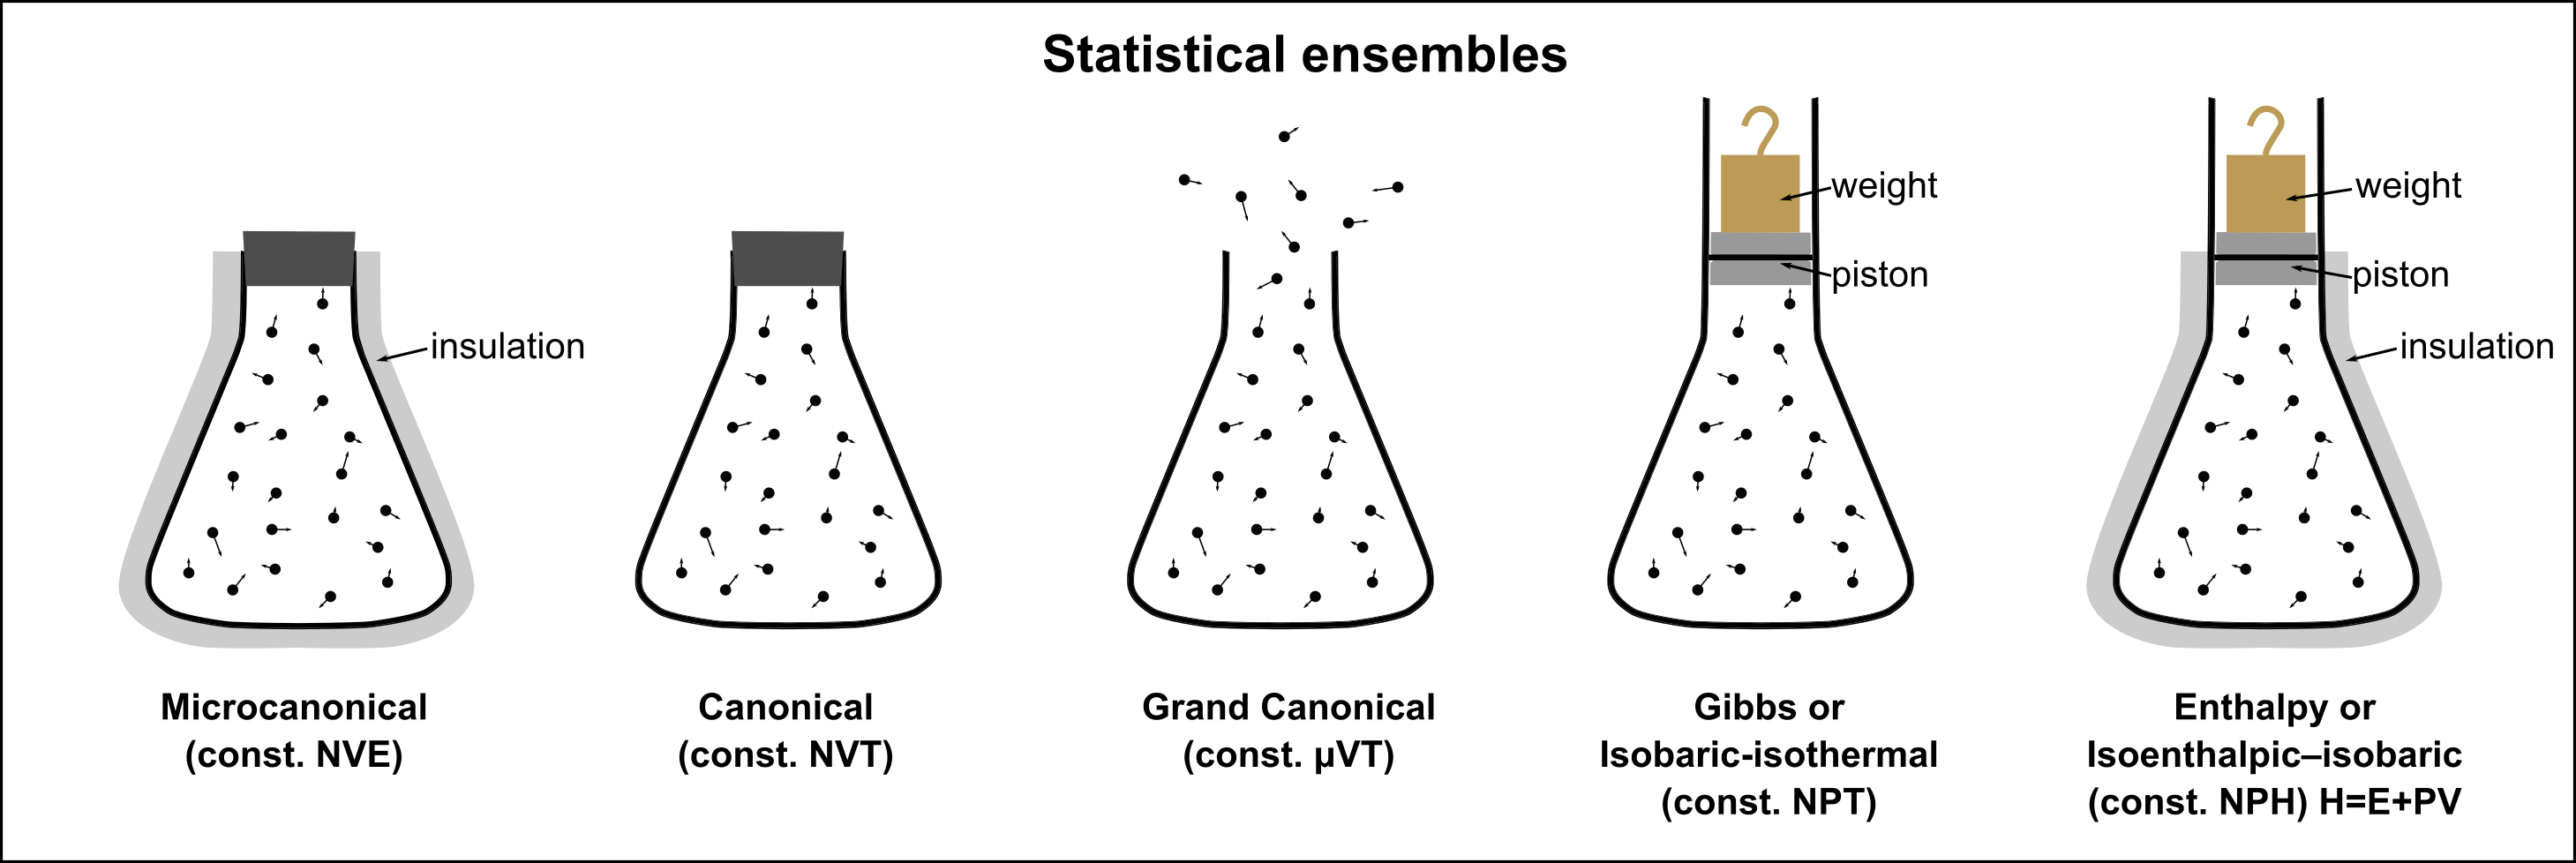
\includegraphics[height=1.20in,width=3.75in,viewport=0 0 1420 470,clip]{Figures/Statistical_Ensembles.png}
\caption{\tiny \textrm{The Statistical Ensembles.}}%(与文献\cite{EPJB33-47_2003}图1对比)
\label{Statistical_Ensembles}
\end{figure}
\vskip -15pt
\begin{itemize}
		{\fontsize{7.2pt}{1.2pt}\selectfont{
		\item 微正则系综\textrm{(Mircocanonical Ensemble)}\footnote{\fontsize{4.5pt}{1.2pt}\selectfont{\textrm{canonical},汉译作``正则'',出自《楚辞\textperiodcentered 离骚》``皇揽揆余於初度兮,肇锡余以嘉名;~名余曰\textcolor{red}{正则}兮,字余曰灵均'',《楚辞章句》\upcite{Chucizhangju}:~``正,平也;~则,法也;~灵,神也;~均,调也。言正平可法则者,莫过于天;~养物均调者,莫神于地。高平曰原,故父伯庸名我为平以法天,字我为原以法地。言己上之能安君,下之能养民也。''意思是说``正则''、``灵均''隐喻着某种意义,即平正是天的象征,原均是地的象征。因此正则的含义是``\textcolor{blue}{符合天道}'',与\textrm{canonical}的意思\textrm{of, relating to, or forming a canon}意义一致。}}:~\textrm{NVE}皆为常数
		\item 正则系综\textrm{(Canonical Ensemble)}:~\textrm{NVT}皆为常数
		\item 巨正则系综\textrm{(Grandcanonical Ensemble)}:~\textrm{$\mu$VT}皆为常数,粒子数不固定
		\item 等压-等温系综\textrm{(Isobaric-Isothermal Ensemble)}:~\textrm{NPT}皆为常数
		\item 等焓-等压系综\textrm{(Isoenthalpic-Isobaric Ensemble)}:~\textrm{NPH}皆为常数
		\item 等张力-等温系综\textrm{(Isotension-Isothermal Ensemble)}:~容器形状可变 }}
\end{itemize}
}

\frame
{
	\frametitle{常用热力学量}
	\begin{itemize}
{\fontsize{7.8pt}{1.2pt}\selectfont{
		\item 动能 ~$E_{\mathrm{k}}=\bigg\langle\sum\limits_{i=1}^N\dfrac12m_iv_i^2\bigg\rangle$
		\item 势能 ~$E_{\mathrm{p}}=\bigg\langle\sum\limits_{i=1}^NE_{\mathrm{p}i}\bigg\rangle$
		\item 温度 ~$T=\dfrac1{\mathrm{d}Nk_{\mathrm{B}}}\bigg\langle\sum\limits_{i=1}^Nm_iv_i^2\bigg\rangle$ ~~~~ 其中$\mathrm{d}$是空间维度
		\item 压强 ~$p=\dfrac{k_{\mathrm{B}}TN}{V}+\dfrac1{\mathrm{d}V}\bigg\langle\sum\limits_{i<j}\vec f_{ij}\cdot\vec r_{ij}\bigg\rangle$
		\item 焓 ~$H=E+pV$ ~~~~ 相当于\textrm{NPT}下的有效总内能
		\item 熵 ~$S=k_{\mathrm{B}}\ln\Omega(N,V,E)$ ~~~~ $\Omega$是系统的总的微观状态数
		\item \textrm{Helmholtz}自由能:~\textcolor{blue}{\textrm{NVT}下的自由能}
			\begin{displaymath}
				F=E-TS=-k_{\mathrm{B}}T\ln{Q}
			\end{displaymath}
		\item \textrm{Gibbs}自由能:~\textcolor{blue}{\textrm{NPT}下的自由能}
			\begin{displaymath}
				G=F+pV=E-TS+pV
			\end{displaymath}
		\item 化学势 ~$\mu=\dfrac{\partial G}{\partial N}\bigg|_{T,p}=\dfrac{\partial F}{\partial N}\bigg|_{T,V}$}}
	\end{itemize}
}

\frame
{
	\frametitle{\textrm{Car-Parrinello~}方法}
	基于\textrm{Born-Oppenheimer}近似的原子-电子耦合的势能面计算,因每一原子步都需要完整的电子结构自洽迭代,故计算量非常可观。
\vskip 5pt
\textrm{1985}年,在\textrm{Car-Parrinello}给出的方案中,\textcolor{purple}{电子态将和原子核的运动一样,都用分子动力学算法处理}\\
在该方案中,\textcolor{blue}{体系的电子态并未能达到当前正电荷环境的真实基态,但体系总能可以与真实基态更为接近}\\
{\fontsize{6.2pt}{5.2pt}\selectfont{考虑\textcolor{blue}{电子态总能}(即\textcolor{red}{电子态有关能量}+\textcolor{magenta}{原子核静电相互作用能})是作为电子波函数$\psi_k$和原子核坐标$\mathbf{S}$的泛函
\begin{displaymath}
	E_{\mathrm{tot}}=E_{\mathrm{tot}}(\{\psi_k\},\mathbf{S})
\end{displaymath}
如果波函数可用一套基组$\{\chi_r\}$表示,即
\begin{displaymath}
	\psi_k(\vec r)=\sum_rC_{rk}\chi_r(\vec r)
\end{displaymath}
则体系总能可表示为
\begin{displaymath}
	E_{\mathrm{tot}}=E_{\mathrm{tot}}(\{C_{rk}\},\mathbf{S})
\end{displaymath}
考虑到基函数常常选择以原子核为坐标原点,因此也依赖于$\mathbf{S}$
}}\\
\textrm{Car-Parrinello}方法通过变量\underline{\textcolor{blue}{$\psi_k$(或$C_{rk}$)和原子核坐标$\mathbf{S}$}}来完成$E_{\mathrm{tot}}$的优化(确定$E_{\mathrm{tot}}$的极小值)
}

\frame
{
	\frametitle{\textrm{Car-Parrinello~}方法}
	{\fontsize{6.2pt}{5.2pt}\selectfont{到这里,能量最小化问题可以视为一个抽象的数学问题,原则上,任何一种最小化方法都适用(如模拟退火方法(\textrm{simulated annealing method}))}}
	\vskip 5pt
	\textrm{Car-Parrinello}要求原子核坐标随时间变化,还引入虚拟时间,要求波函数随虚拟时间变化,由此构造动态\textrm{Lagrangian}量\\
	{\fontsize{6.2pt}{5.2pt}\selectfont{\textrm{Lagrangian}量包括
	\begin{itemize}
		\item 电子态波函数$\{\psi_k\}$
		\item 原子核坐标$\{\vec R_i\}$
		\item 电子态波函数时间导数$\dot\psi_k$和原子核坐标时间导数$\{\dot{\vec R}_i\}$
	\end{itemize}}}
	电子态总能$E_{\mathrm{tot}}$是该\textrm{Lagrangian}量的势能,形式上这是一个经典力学的问题
	\begin{itemize}
		\item 在经典力学体系的运动方程中引入阻尼项贡献,则\\
			\textcolor{blue}{经过一段时间体系达到平衡态时,许可自由度的值对应体系经典势能达到最小值态时的取值}
		\item 在模拟体系在非零温下的运动时,可将阻尼项设为零
	\end{itemize}
}

\frame
{
	\frametitle{\textrm{Car-Parrinello}的\textrm{Lagrangian}}
	根据\textrm{Car-Parrinello~}定义的经典\textrm{Lagrangian~}量
	{\fontsize{9.0pt}{5.2pt}\selectfont
	\begin{displaymath}
		L(\{\psi_k\},\{\vec R_n\})=\frac{\mu}2\sum_k\dot{\psi}_k^2+\sum_n\frac{M_n}2\dot{\vec R}_n^2-E_{\mathrm{tot}}(\{\psi_k\},\{\vec R_n\})+\sum_{kl}\Lambda_{kl}\langle\psi_k|\psi_l\rangle
	\end{displaymath}}
	这里$\mu$是一个很小的质量(可理解为虚拟电子质量);\\
	$M_n$表示位置为$\vec R_n$处原子的真实质量;~\\
	上式最后一项是要求波函数$\psi_k$正交的约束条件,$\Lambda_{kl}$是引入的\textrm{Lagrangian}乘子
\vskip 5pt
{\fontsize{7.2pt}{5.2pt}\selectfont{$\mu$的选择原则:
		\begin{enumerate}
			\item $\mu\ll M$:~使得\textrm{Lagrangian}量中的\textcolor{blue}{电子动能项贡献足够小},因此波函数能随时适应原子核位置的变化
			\item $\mu$的选择兼顾效率与精度:\\
				一旦在运动方程中引入阻尼,电子和原子核的动能都将为零,体系总能(即\textrm{Lagrangian}量中的势能)达到极小值,但选择不同的$\mu$,计算过程中会有不同的收敛速度
		\end{enumerate}
	}}
}

\frame
{
	\frametitle{运动方程}
由波函数正交约束,体系的\textrm{Euler-Lagrange~}运动方程可表示为
	\begin{displaymath}
		\begin{aligned}
			\mu\ddot{\psi}_k=&-\dfrac{\partial E_{\mathrm{tot}}}{\partial\psi_k}+2\sum_i\Lambda_{kl}(t)\psi_l(\vec r)\\
			M_n\ddot{\vec R}_n&=-\dfrac{\partial E_{\mathrm{tot}}}{\partial\vec R_n}+\textcolor{red}{\sum_{kl}\Lambda_{kl}(t)\dfrac{\partial\langle\psi_k|\psi_l\rangle}{\partial\vec R_n}}
		\end{aligned}
	\end{displaymath}
	{\fontsize{7.2pt}{5.2pt}\selectfont{\begin{itemize}
		\item \textcolor{red}{如果表示$\psi_k$的基函数不依赖原子核位置$\mathbf{S}$,则上述最后一个方程右侧最后一项消失}
		\item 电子态总能$E_{\mathrm{tot}}$是波函数$\psi_k$和原子核位置$\{\vec R_n\}$的函数
		\item 当波函数用基函数展开,电子运动方程可用展开系数表示为
			\begin{displaymath}
				\mu\ddot{\psi}_k=-\dfrac{\partial E_{\mathrm{tot}}}{\partial\psi_k}+2\sum_i\Lambda_{kl}(t)\sum_sS_{rs}(\vec r)C_{sl}
			\end{displaymath}
%		只要电子态波函数的基函数可由原子核位置确定,$\mu$的数值受基函数影响不大
	\end{itemize}}}
}

\frame
{
	\frametitle{定态运动方程的求解}
	如果运动方程中引入阻尼项,则经过一段时间后,方程的解达到定态,前述运动方程等号左侧为零\footnote{\fontsize{6.2pt}{5.2pt}\selectfont{定态,意味着波函数和原子位置不再随时间变化}},因此可有
\begin{itemize}
	\item 电子态的运动方程与\textrm{Kohn-Sham}方程类似\\
		{\fontsize{6.2pt}{5.2pt}\selectfont{当前方程的矩阵元$\Lambda_{kl}$与\textrm{K-S}方程的能量本征值由$\varepsilon_k$对应}}
	\item \textrm{Lagrange}参数$\Lambda_{kl}$是时间相关的\\
		{\fontsize{6.2pt}{5.2pt}\selectfont{
		因此每个\textrm{MD}步必须重新计算$\Lambda_{kl}$,确保电子态波函数满足正交约束条件}}
	\item 应用具体的数值算法求解$\Lambda_{kl}$:~\\
	{\fontsize{6.5pt}{5.2pt}\selectfont
	应用\textrm{DFT~}框架下的\textrm{Hamiltonian}量,有
	\begin{displaymath}
		\psi_k(t+h)=2\psi_k(t)-\psi_k(t-h)-\dfrac{2h^2}{\mu}(H\psi_k-\sum_l\Lambda_{kl}\psi_l)
	\end{displaymath}
	该方程表明:~\textcolor{blue}{电子基态也可通过各种优化方法直接求解}}\\
		{\fontsize{6.2pt}{5.2pt}\selectfont{
			比如可用\textrm{Verlet~}算法计算;~\textrm{Car-Parrinello}建议用迭代\textrm{SHAKE}算法计算}}
	\item 对于搜索原子核的平衡位置问题,如果原子初始位置离平衡位置较远,很可能只得到体系的局域极小值\\
		{\fontsize{6.2pt}{5.2pt}\selectfont{使用模拟退火方法,使体系跃出局域极小点,搜索全局极小值}}
\end{itemize}
}

%\frame
%{
%	\frametitle{能量泛函的直接优化:~波函数的求解}
%	在\textrm{DFT~}框架下,有
%	{\fontsize{9.0pt}{5.2pt}\selectfont
%	\begin{displaymath}
%		\psi_k(t+h)=2\psi_k(t)-\psi_k(t-h)-\dfrac{2h^2}{\mu}(H\psi_k-\sum_l\Lambda_{kl}\psi_l)
%	\end{displaymath}}
%%	该方程表明:~\textcolor{blue}{电子基态也可通过各种优化方法直接求解}
%	每个时间步$t$,\textrm{Car-Parrinello~}采用\textrm{SHAKE~}算法迭代确定$\psi_k(t)$
%}
%
\frame
{
	\frametitle{原子核受力}
	原子核运动方程的求解主要围绕电子态总能对原子位置$\vec R_i$的求导,对求导有贡献的共三部分
	\begin{itemize}
		\item 原子核之间的\textrm{Coulomb}相互作用:\\
			与原子核间距离反比:~$1/R_{ij}~\quad|\vec R_{ij}=\vec R_i-\vec R_j|$
		\item 电子\textrm{Hamiltonian}中包括的电子与核之间的\textrm{Coulomb}吸引势\\
			与原子核位置有关:~$\vec R_i$
		\item 基函数$\chi_r$对原子核位置$\vec R_i$的依赖\\
			当基函数的中心选定在原子核$\vec R_i$上时,原子核位置的变化会引起\textrm{Fock}矩阵和重叠矩阵的变化\\
	{\fontsize{7.2pt}{5.2pt}\selectfont{因原子核位置变化引起基函数改变的贡献称为\textcolor{blue}{\textrm{Pulay}力}}}
	\end{itemize}
	\textrm{Car-Parrinello}方法得到的结果与二体势(力场)方法结果等价
	\vskip 5pt
	计算得到位于$\vec R_i$的原子核受力,用于描述\textrm{Verlet}模拟原子核的运动状态
}

\frame
{
	\frametitle{\textrm{H}原子\textrm{AIMD}计算示例}
\begin{figure}[h!]
	\vspace{-0.25in}
\centering
%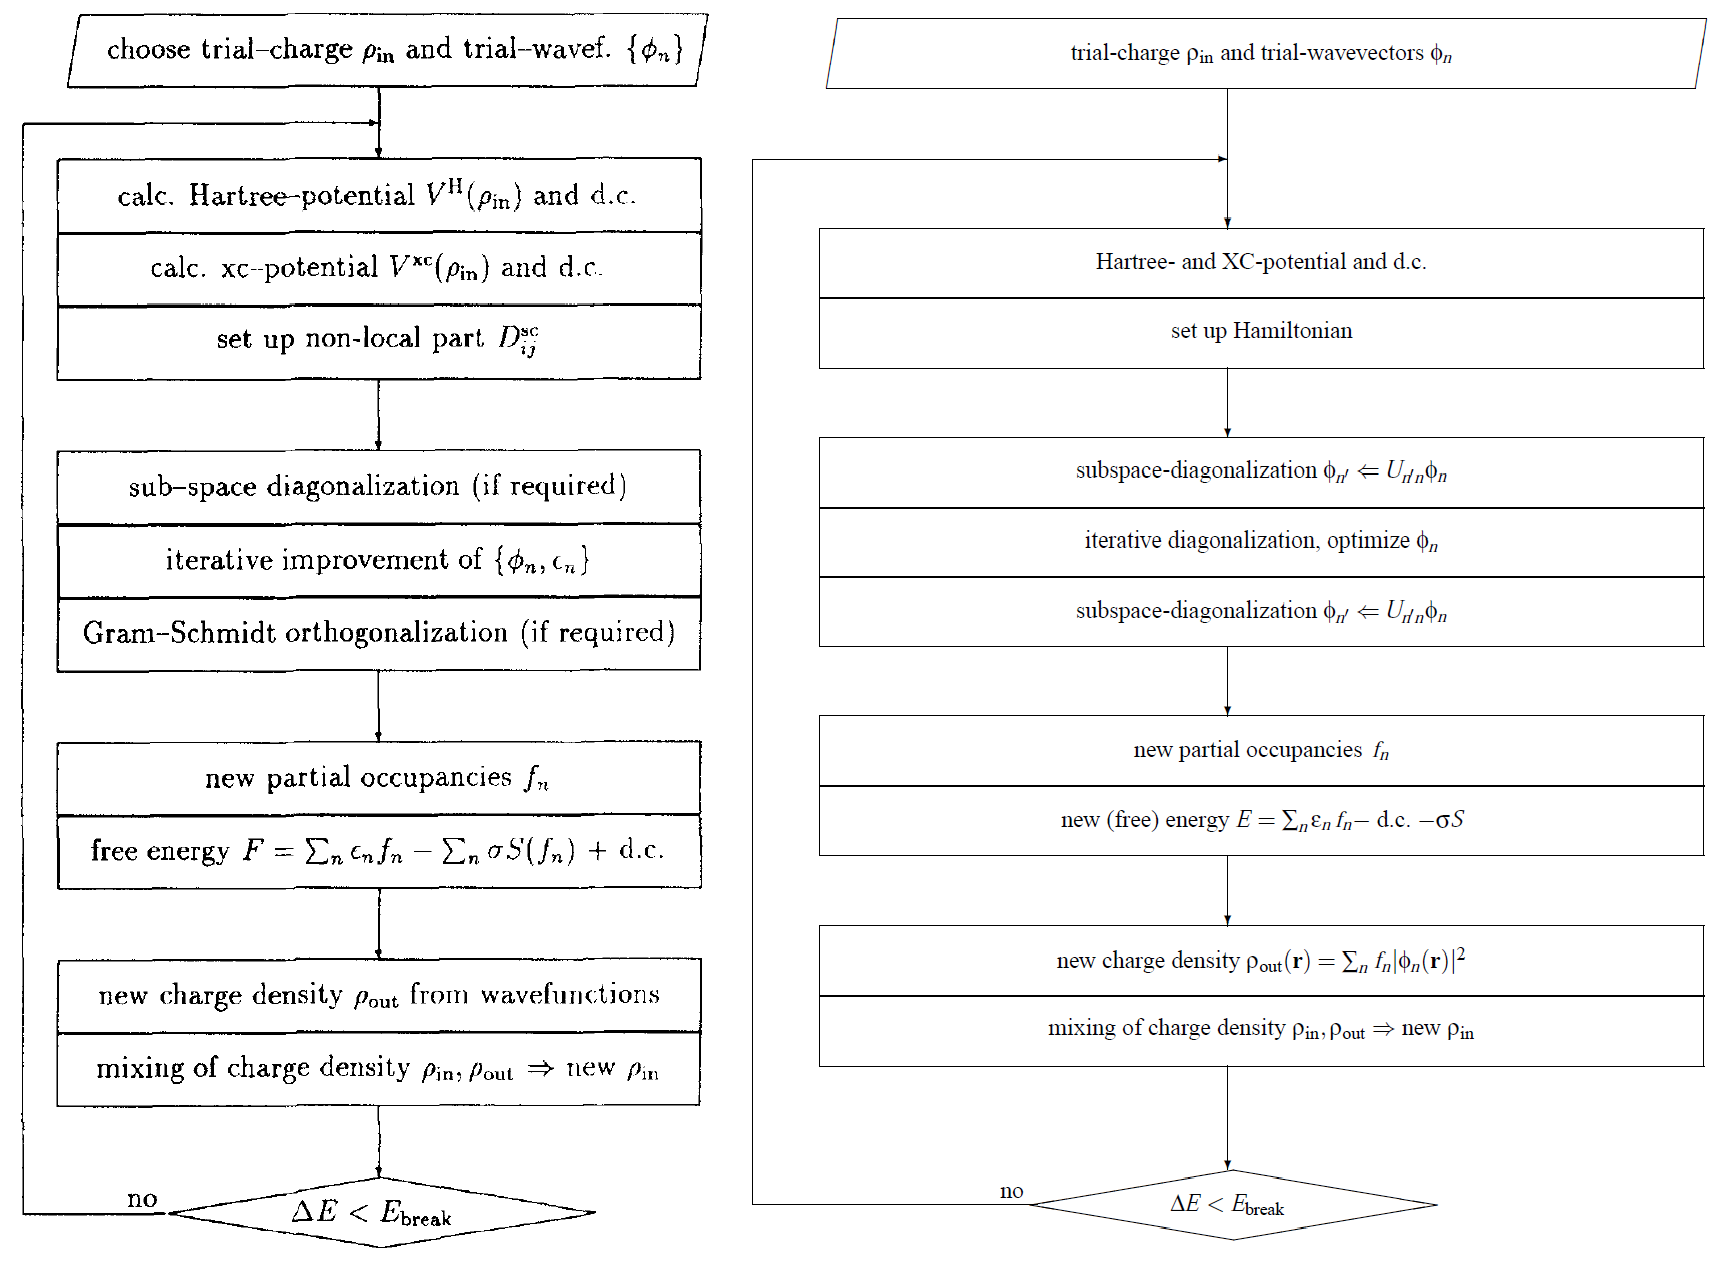
\includegraphics[height=2.7in,width=4.0in,viewport=0 0 1300 960,clip]{Figures/VASP_procedure-full.png}
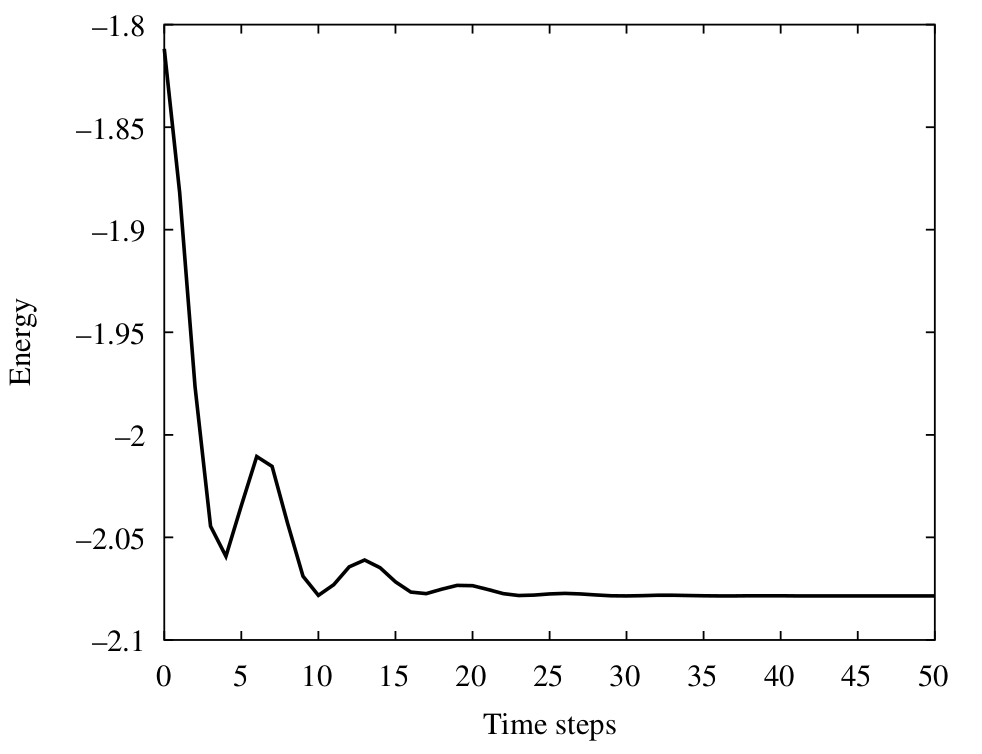
\includegraphics[height=1.5in,width=1.9in,viewport=0 0 740 600,clip]{Figures/Ab-initio-Ene.png}\\
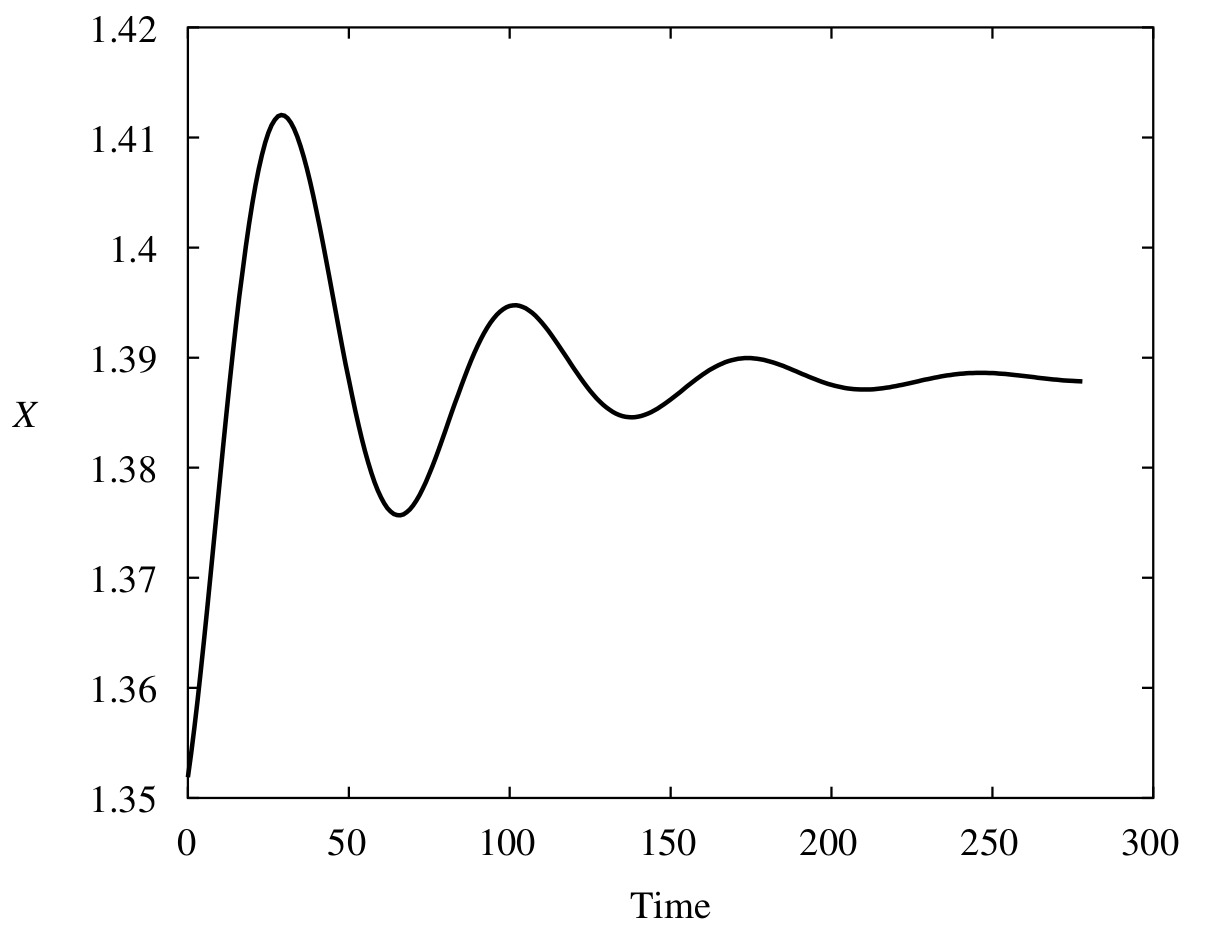
\includegraphics[height=1.5in,width=1.9in,viewport=0 0 1200 950,clip]{Figures/MD_H-R-rel.png}
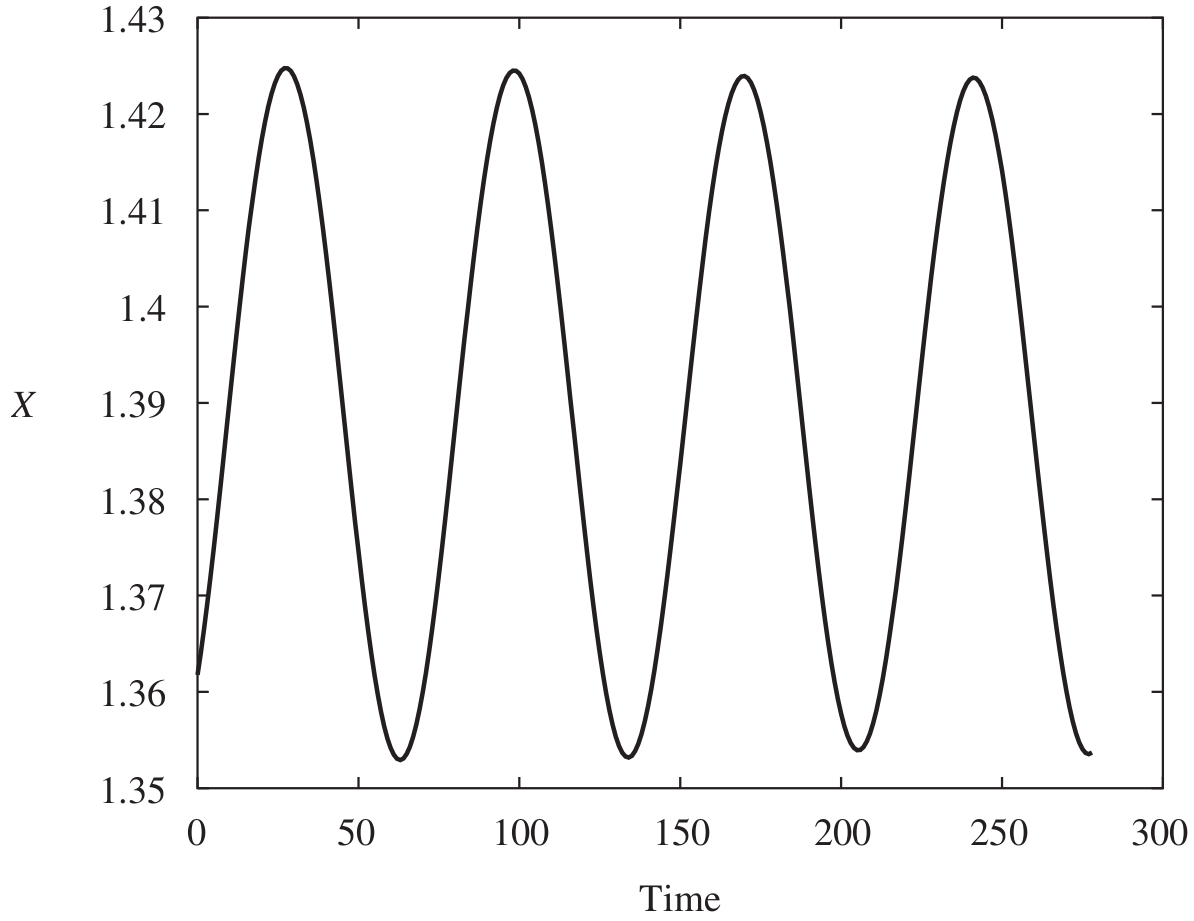
\includegraphics[height=1.5in,width=1.9in,viewport=0 0 1200 950,clip]{Figures/MD_H-R-MD.png}
\caption{\tiny \textrm{The Flow of calculation for the AIMD.}}%(与文献\cite{EPJB33-47_2003}图1对比)
\label{PAW_AIMD}
\end{figure} 
}


\frame
{
	\frametitle{波函数正交对计算的影响}
	{\fontsize{9.0pt}{5.2pt}\selectfont
	\textrm{Verlet}算法计算电子态波函数的运动方程
	\begin{displaymath}
		|\tilde\psi_k(t+h)\rangle=2|\psi_k(t)\rangle-|\psi_k(t-h)\rangle-\dfrac{2h^2}{\mu}(H|\psi_k(t)\rangle-\sum_l\Lambda_{kl}\psi_l)
	\end{displaymath}}
	当体系含有多个电子,\textrm{Langrage}乘子确保电子波函数彼此正交\\%,可有
	{\fontsize{7.0pt}{5.2pt}\selectfont
	实际上,存在多种正交方案
	\begin{itemize}
		\item 一次\textrm{unitary}变换产生一套正交轨道
			\begin{displaymath}
				\psi_k^{\prime}=\sum_lU_{kl}\psi_l
			\end{displaymath}
			这里基组$\{\psi_k^{\prime}\}$是正交的
		\item 一次波函数的\textrm{unitary}变化伴随\textrm{Lagtange}乘子的一次类似变换
			\begin{displaymath}
				\Lambda_{kl}^{\prime}=\sum_{mn}U_{km}^{\dagger}\Lambda_{mn}U_{nl}
			\end{displaymath}
	\end{itemize}
	不同的正交方案对应张开的空间相同,但张开空间的函数有所旋转
%	\begin{displaymath}
%		|\psi_k(t+h)\rangle=|\tilde\psi_k(t+h)\rangle+\sum_lX_{kl}|\psi_l(t)\rangle
%	\end{displaymath}
}\\
%	其中,{\fontsize{9.0pt}{5.2pt}\selectfont$X_{kl}=\dfrac{2h^2}{\mu}\Lambda_{kl}$},由此$|\psi_k(t+h)\rangle$正交\\
%	$X_{ij}$要求关于$\mathbf{X}$的矩阵方程
	{\fontsize{8.0pt}{5.2pt}\selectfont
	\textcolor{purple}{不同的旋转方式(不同的正交方案)会对\textrm{Verlet}算法的执行效率产生很大的影响}
%	\begin{displaymath}
%		\mathbf{X}\mathbf{X}^{\dag}+\mathbf{X}\mathbf{B}+\mathbf{B}^{\dag}\mathbf{X}^{\dag}=\mathbf{I}-\mathbf{A}
%	\end{displaymath}
}
%	能通过以下迭代快速收敛,这里{\fontsize{9.0pt}{5.2pt}\selectfont$A_{kl}=\langle\tilde\psi_k(t+h)|\tilde\psi_l(t+h)\rangle$},{\fontsize{9.0pt}{5.2pt}\selectfont$B_{kl}=\langle\psi_k(t)|\tilde\psi_l(t+h)\rangle$}
	{\fontsize{9.0pt}{5.2pt}\selectfont
%	\begin{displaymath}
%		\mathbf{X}^{(n+1)}=\frac12[\mathbf{I}-\mathbf{A}+\mathbf{X}^{(n)}(\mathbf{I}-\mathbf{B})+\mathbf{X}^{(n)}(\mathbf{I}-\mathbf{B}^{\dag})-\mathbf{X}^{n}\mathbf{X}^{(n){\dag}}]
%		\end{displaymath}
}
%	取初始{\fontsize{9.0pt}{5.2pt}\selectfont$\mathbf{X}=\frac12(\mathbf{I}-\mathbf{A})$}
}

%\subsection{电子态能量的最小化}
\frame[allowframebreaks]
{
	\frametitle{\textrm{Car-Parrinello}方法与平面波基}
	\begin{itemize}
		\item 推导总能对轨道自由度的受力
	{\fontsize{6.2pt}{5.2pt}\selectfont{
			\begin{displaymath}
				\begin{aligned}
					\dfrac{\partial E_{\mathrm{total}}}{\partial c_j^{\ast}(\vec K)}=&\dfrac{K^2}2c_j(\vec K)+\sum_{\vec K^{\prime}}V_{\mathrm{loc}}^{\ast}(\vec K-\vec K^{\prime})c_j(\vec K^{\prime})\\
					&+\sum_n\sum_{lm}F_{jlm}^n\mathrm{e}^{-\mathrm{i}\vec K\cdot\vec R_n}Y_{lm}(\hat{\vec K})h_{lm}^np_m^l(K)
				\end{aligned}
			\end{displaymath}
			这里$V_{\mathrm{loc}^{\mathrm{all}}}$是总局域势
			\begin{displaymath}
				V_{loc}(\vec K)=\sum_n\Delta V_{\mathrm{loc}}(\vec K)+V_{\mathrm{xc}}(\vec K)+4\pi\dfrac{n_{\mathrm{tot}}(\vec K)}{K^2}
			\end{displaymath}
		}}
		\item 推导总能对原子核的受力:\\
{\fontsize{6.2pt}{5.2pt}\selectfont{
			总能对原子位置坐标的梯度包括
			\begin{itemize}
{\fontsize{6.2pt}{5.2pt}\selectfont{
				\item 局域赝势部分的贡献
					\begin{displaymath}
						\nabla_{\vec R_n}E_{\mathrm{local}}=-\Omega\sum_{\vec K}\mathrm{i}\vec KV_{\mathrm{local,n}}(\vec K)\mathrm{e}^{-\mathrm{i}\vec K\cdot\vec R_n}n^{\ast}(\vec K)
					\end{displaymath}
				\item 非局域赝势部分的贡献
					\begin{displaymath}
						\nabla_{\vec R_n}E_{\mathrm{nonlocal}}=\sum_jf_j\sum_{l,m\varepsilon n}[(F_{jlm}^n)^{\ast}h_{lm}^n\nabla_{\vec R_n}F_{jlm}^n+\nabla_{\vec R_n}(F_{lm}^n)^{\ast}h_{lm}^nF_{lm}^n]
					\end{displaymath}
				\item 电子-核静电相互作用部分的贡献
					\begin{displaymath}
						\nabla_{\vec R_n}E_{\mathrm{ES}}=-\Omega\sum_{\vec K}\mathrm{i}\vec K\dfrac{n_{\mathrm{tot}}}{K^2}n_{\mathrm{core}}^n(\vec K)\mathrm{e}^{-\mathrm{i}\vec K\cdot\vec R_n}+\nabla_{\vec R_n}E_{\mathrm{ovrl}}
\end{displaymath}
				}}
			\end{itemize}
			其中
			\begin{displaymath}
				\nabla_{\vec R_n}F_{lm}^n=-\dfrac1{\sqrt{\Omega}}\sum_{\vec K}\mathrm{i}\vec K\mathrm{e}^{-\mathrm{i}\vec K\cdot\vec R_n}c_j^{\ast}(\vec K)Y_{lm}(\hat{\vec K})p_{lm}^l(\vec K)
			\end{displaymath}
			\begin{displaymath}
				\begin{aligned}
					\nabla_{\vec R_n}E_{\mathrm{ovrl}}=&\sideset{}{^{\prime}}\sum_{n^{\prime}}\sum_{\vec L}\bigg\{\dfrac{Z_nZ_{n^{\prime}}}{|\vec R_n-\vec R_{n^{\prime}}-\vec L|^3}\mathrm{erfc}\bigg[\dfrac{|\vec R_n-\vec R_{n^{\prime}}-\vec L|}{\sqrt{2(\xi_n^2+\xi_{n^{\prime}}^2)}}\bigg]\\
					&+\dfrac2{\sqrt{\pi}}\dfrac1{\sqrt{\xi_n^2+\xi_{n^{\prime}}^2}}\dfrac{Z_nZ_{n^{\prime}}}{|\vec R_n-\vec R_{n^{\prime}}-\vec L|^2}\mathrm{exp}\bigg[\dfrac{|\vec R_n-\vec R_{n^{\prime}}-\vec L|}{\sqrt{2(\xi_n^2+\xi_{n^{\prime}}^2)}}\bigg]\bigg\}\\
					&\times(\vec R_n-\vec R_{n^{\prime}}-\vec L)
				\end{aligned}
			\end{displaymath}
		}}
	\end{itemize}

}

\frame
{
	\frametitle{第一原理分子动力学提要}
	\textrm{Car-Parinello~}方法基本思想
	\begin{itemize}
		\item 只对原子核位置考虑受力$-\dfrac{\partial E_{\mathrm{tot}}}{\partial\vec R_n}$作用
		\item 电子结构是通过某种最小化方法确定能量泛函$E_{\mathrm{tot}}[\rho(\vec r)]$的极值得到,而非\textrm{Born-Oppenheimer}近似下的自洽迭代
		\item \textrm{Verlet}算法确定核位移过程中,并不要求在每一步核位移时,电子步充分弛豫到当前结构的基态
	\end{itemize}
	在\textrm{Car-Parinello}方法中,电子结构的计算变成经典的优化问题:~电子密度迭代过程中,约束条件下最小化问题
	\begin{itemize}
		\item 电子本征态波函数彼此正交约束下迭代对角化(内循环):\\
			\textcolor{blue}{子空间旋转}:~不同的正交化方法对迭代计算的影响
		\item 电荷密度混合过程中电荷数守恒约束(外循环)
			\begin{displaymath}
				\sum\limits_{j=0}^i a_j=1
			\end{displaymath}
	\end{itemize}
}

%------------------------------------------------------------------------Reference----------------------------------------------------------------------------------------------
		\frame[allowframebreaks]
{
\frametitle{主要参考文献}
\begin{thebibliography}{99}
{\tiny
	\bibitem{CMS6-15_1996}\textrm{G. Kresse and J. Furthm\"uller \textit{Comput. Mat. Sci.}, \textbf{6} (1996), 15}
	\bibitem{PRB54-11169_1996}\textrm{G. Kresse and J. Furthm\"uller \textit{Phys. Rev.} B, \textbf{54} (1996), 11169}
	\bibitem{PRL55-2471_1985}\textrm{R. Car and M. Parrinello \textit{Phys. Rev.} Lett., \textbf{55} (1985), 2471}
	\bibitem{PRB47-10142_1993}\textrm{K. Laasonen and A. Pasquarello and R. Car and C. Lee and D. Vanderbilt \textit{Phys. Rev.} B, \textbf{47} (1993), 10142}
	\bibitem{Chucizhangju}[东汉]王逸~撰. \textit{楚辞章句}\:上海古籍出版社, 上海, 2017
	\bibitem{Elect_Stru}\textrm{Richard. M. Martin. \textit{Electronic Structure: Basic Theory and Practical Methods} (Cambridge University Press, Cambridge, England, 2004)}
	\bibitem{Comp_Phys}\textrm{J. M. Thijssen. \textit{Computational Physics (2nd Edition)} (Cambridge University Press, Cambridge, England, 2007)}
        \bibitem{Singh}\textrm{D. J. Singh. \textit{Plane Wave, PseudoPotential and the LAPW method} (Kluwer Academic, Boston,USA, 1994)}					%
}
\end{thebibliography}
%\nocite*{}
}
%-----------------------------------------------------------------------------------------------------------------------------------------------------------------------%
